\documentclass[12pt]{article}
\usepackage[T1]{fontenc}
\usepackage[T1]{polski}
\usepackage[utf8]{inputenc}
\usepackage{graphicx}
\usepackage{amsfonts}
\usepackage{float}

\setlength{\textheight}{20cm}

\title{{\bf Zadanie nr1 - Generacja sygnału i
szumu}\linebreak
Cyfrowe Przetwarzanie Sygnałów}
\author{Krzysztof Barden, 210139 \and Paweł Galewicz, 210182}
\date{29.03.2019r.}

\begin{document}
\clearpage\maketitle
\thispagestyle{empty}
\newpage
\setcounter{page}{1}
\section{Cel zadania}

Celem zadania jest zapoznanie się z wybranymi własnosciami podstawowych
rodzajów sygnałów oraz przygotowanie aplikacji je generujące. Sygnały te to:
\begin{itemize}
\item szum o rozkładzie jednostajnym;
\item szym gaussowski;
\item sygnał sinusoidalny;
\item sygnał sinusoidalny wyprostowany jednopołówkowo;
\item sygnał sinusoidalny wyprostowany dwupołówkowo;
\item sygnał prostokątny;
\item sygnał prostokątny symetryczny;
\item sygnał trójkątny;
\item skok jednostkowy;
\item impuls jednostkowy;
\item szum impulsowy;
\end{itemize}
Dodatkową funkcjonalnoscią progamu jest wykonywanie podstawowych dziań na sygnałach:
\begin{itemize}
\item dodawanie;
\item odejmowanie;
\item mnożenie;
\item dzielenie;
\end{itemize}
Możliwe jest też zapisywanie i wczytywanie otrzymanych wykresów z użyciem plików o rozszerzeniu ".sign".
Program wylicza też następujące parametry sygnału:
\begin{itemize}
\item wartość średnią,
\item wartość średnią bezwzględną, 
\item wartość skuteczną, 
\item wariancję,
\item moc średnią.
\end{itemize}

\section{Wstęp teoretyczny}

Program został napisany w języku C\#. Wykresy generowane są przy użyciu biblioteki LiveCharts \cite{lv}. GUI aplikacji zostało stworzone przy użyciu biblioteki WPF \cite{wpf}.
\\Po włączeniu się programu pojawia się dany interfejs:
\begin{figure}[H]
 \centering
 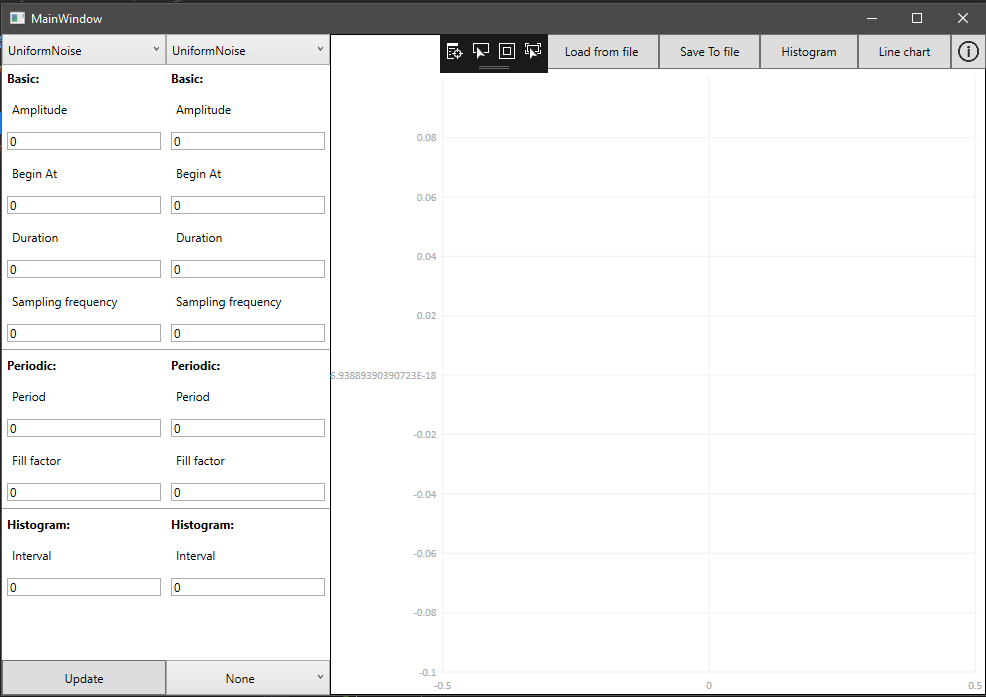
\includegraphics[width=15cm]{images/gui1.PNG}
 \vspace{-0.3cm}
 \caption{Interfejs graficzny użytkownika}
 \label{gui}
\end{figure}

Aby wygenerować sygnał należy w lewej kolumnie wybrać z listy odpowiedni rodzaj sygnału,  wypełnić parametry i nacisnąć przycisk "Update". Aby pokazać histogarm dla danego sygnału należy nacisnąć przycisk "Histogram". Aby zapisać sygnał należy nacisnąć przyciks "Save to file". Aby wczytać sygnał z pliku należy nacisnąć przycisk "Load from File".

By wykonać operacje na dwóch wykresach, należy w lewej i prawej kolumnie wybrać typ wykresu i wypełnić parametry, następnie wybrać z rozwijanej listy (przycisk "None") typ działania (domyslny brak działania) oraz nacisnąć przycisk "Update".

Aby wyswietlić obliczone wartosci należy nacisnąć przycisk w prawym górnym rogu ('i' w kółku).
\section{Eksperymenty i wyniki}


%%%%%%%%%%%%%%%%%%%%%%%%%%%%%%%%%%%%%%%%%%%%%%%%%%%%%%%%%%%%%%%%%%%%%%%%%%%%%%%%%%%%%%%%%%%%%%%%%%%%%%%%%%%%%%%%%
% PODROZDZIAŁ PT. EKSPERYMENT NR 1 
%%%%%%%%%%%%%%%%%%%%%%%%%%%%%%%%%%%%%%%%%%%%%%%%%%%%%%%%%%%%%%%%%%%%%%%%%%%%%%%%%%%%%%%%%%%%%%%%%%%%%%%%%%%%%%%%%

\subsection{Eksperyment nr 1}




\subsubsection{Generowanie sygnału sinusoidalnego}
Celem tego eksperymentu było wygenerowanie sygnału skoku jednostkowego.


\subsubsection{Rezultat}

\begin{figure}[H]
 \centering
 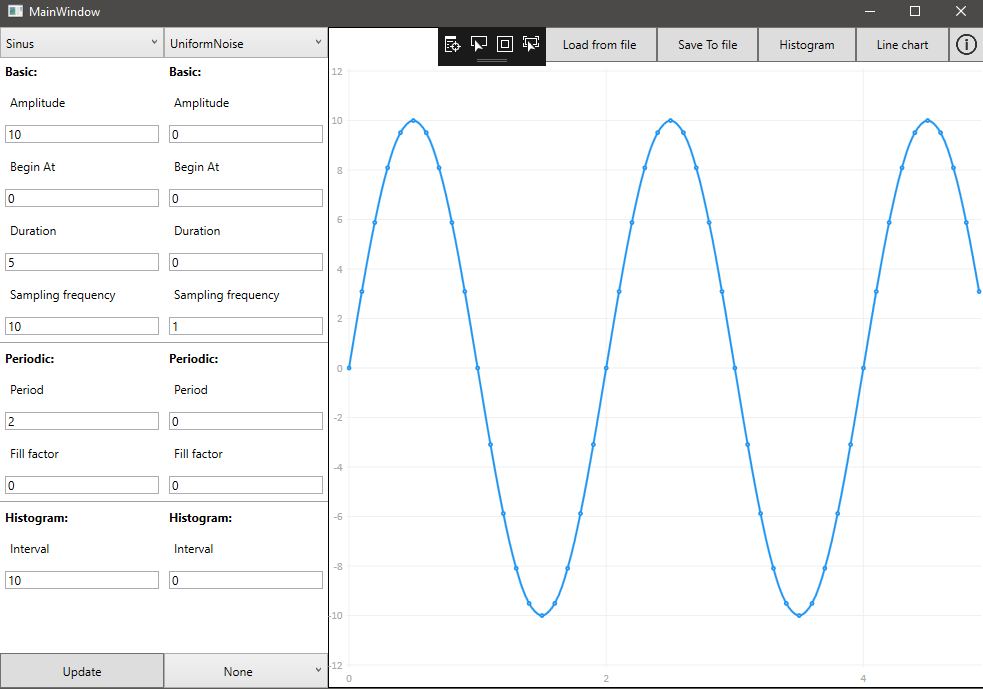
\includegraphics[width=15cm]{images/sin1.PNG}
 \vspace{-0.3cm}
 \caption{Wykres sygnału sinusoidalnego}
 \label{gui}
\end{figure}

\begin{figure}[H]
 \centering
 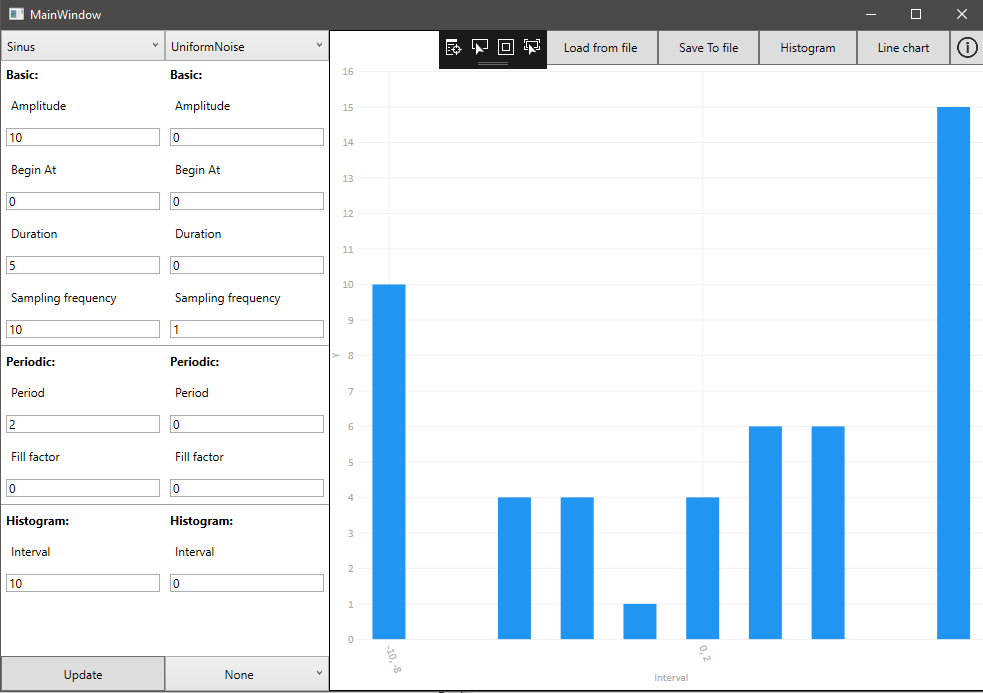
\includegraphics[width=15cm]{images/sin1hist.PNG}
 \vspace{-0.3cm}
 \caption{Histogram dla sygnału sinusoidalnego}
 \label{gui}
\end{figure}

\begin{figure}[H]
 \centering
 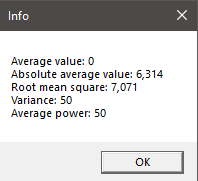
\includegraphics[width=7cm]{images/sin1info.PNG}
 \vspace{-0.3cm}
 \caption{Wyliczone wartosci dla sygnału sinusoidalnego}
 \label{gui}
\end{figure}

%%%%%%%%%%%%%%%%%%%%%%%%%%%%%%%%%%%%%%%%%%%%%%%%%%%%%%%%%%%%%%%%%%%%%%%%%%%%%%%%%%%%%%%%%%%%%%%%%%%%%%%%%%%%%%%%%
% PODROZDZIAŁ PT. EKSPERYMENT NR 2 
%%%%%%%%%%%%%%%%%%%%%%%%%%%%%%%%%%%%%%%%%%%%%%%%%%%%%%%%%%%%%%%%%%%%%%%%%%%%%%%%%%%%%%%%%%%%%%%%%%%%%%%%%%%%%%%%%

\newpage
\subsection{Eksperyment nr 2}
\subsubsection{Generowanie szumu gaussowskiego}
Celem tego eksperymentu było wygenerowanie szumu gaussowskiego.


\subsubsection{Rezultat}

\begin{figure}[H]
 \centering
 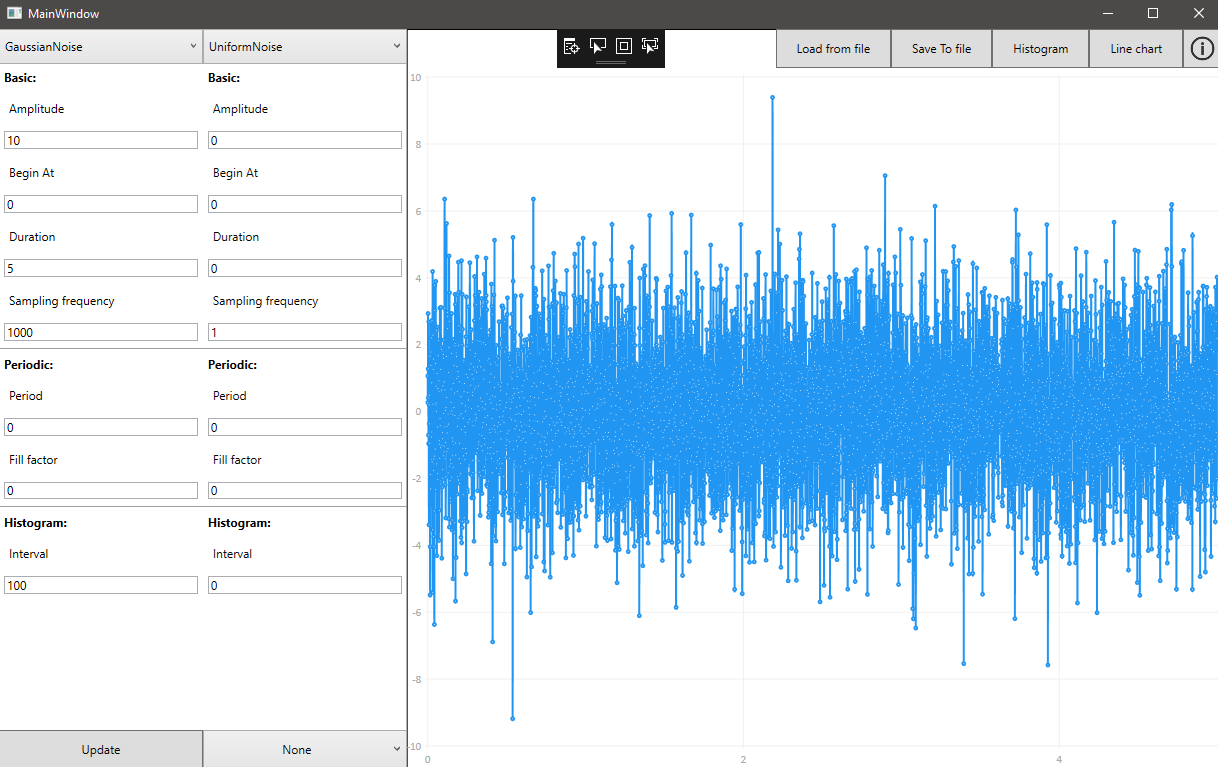
\includegraphics[width=14cm]{images/gauss1.PNG}
 \vspace{-0.3cm}
 \caption{Wykres szumu gaussowskiego}
 \label{gui}
\end{figure}

\begin{figure}[H]
 \centering
 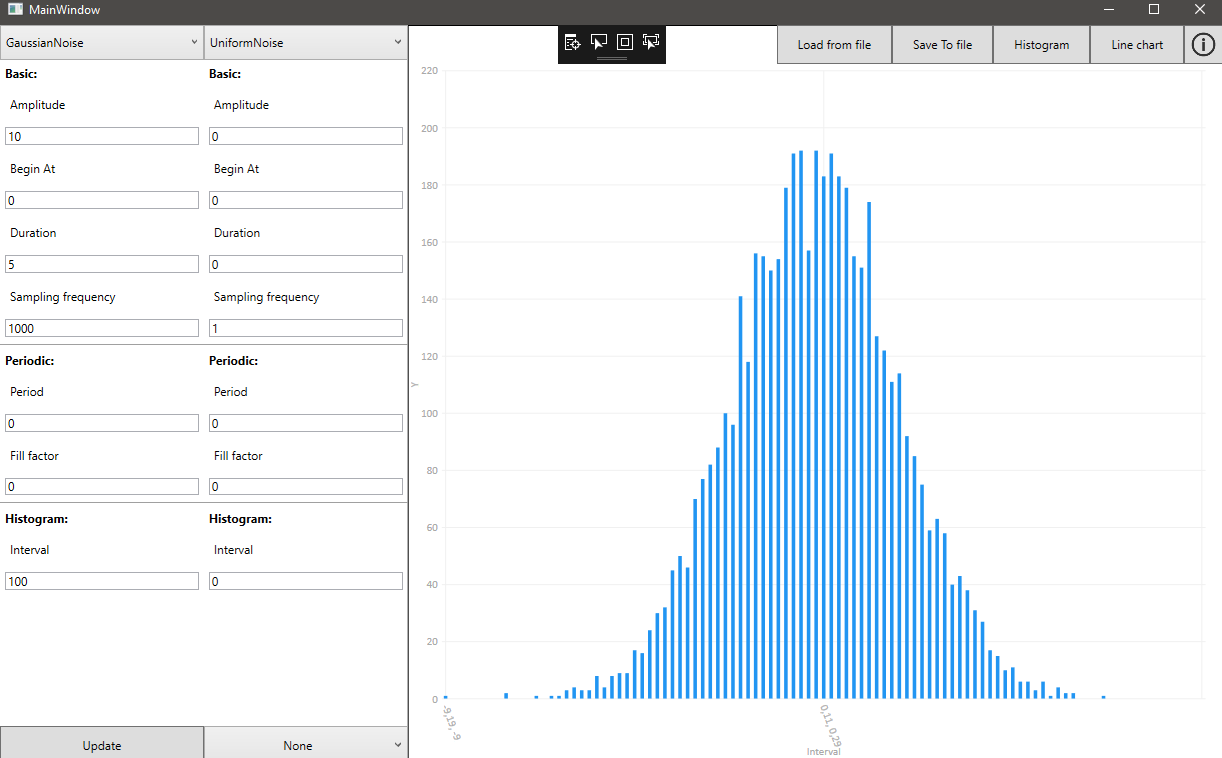
\includegraphics[width=14cm]{images/gauss1hist.PNG}
 \vspace{-0.3cm}
 \caption{Histogram dla szumu gaussowskiego}
 \label{gui}
\end{figure}

\begin{figure}[H]
 \centering
 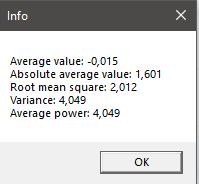
\includegraphics[width=7cm]{images/gauss1info.PNG}
 \vspace{-0.3cm}
 \caption{Wyliczone wartosci dla szumu gaussowskiego}
 \label{gui}
\end{figure}

%%%%%%%%%%%%%%%%%%%%%%%%%%%%%%%%%%%%%%%%%%%%%%%%%%%%%%%%%%%%%%%%%%%%%%%%%%%%%%%%%%%%%%%%%%%%%%%%%%%%%%%%%%%%%%%%%
% PODROZDZIAŁ PT. EKSPERYMENT NR 3 
%%%%%%%%%%%%%%%%%%%%%%%%%%%%%%%%%%%%%%%%%%%%%%%%%%%%%%%%%%%%%%%%%%%%%%%%%%%%%%%%%%%%%%%%%%%%%%%%%%%%%%%%%%%%%%%%%


\subsection{Eksperyment nr 3 }
\subsubsection{Generowanie szumu o rozkladzie jednostajnym}
Celem tego eksperymentu było wygenerowanie szumu o rozkladzie jednostajnym.


\subsubsection{Rezultat}

\begin{figure}[H]
 \centering
 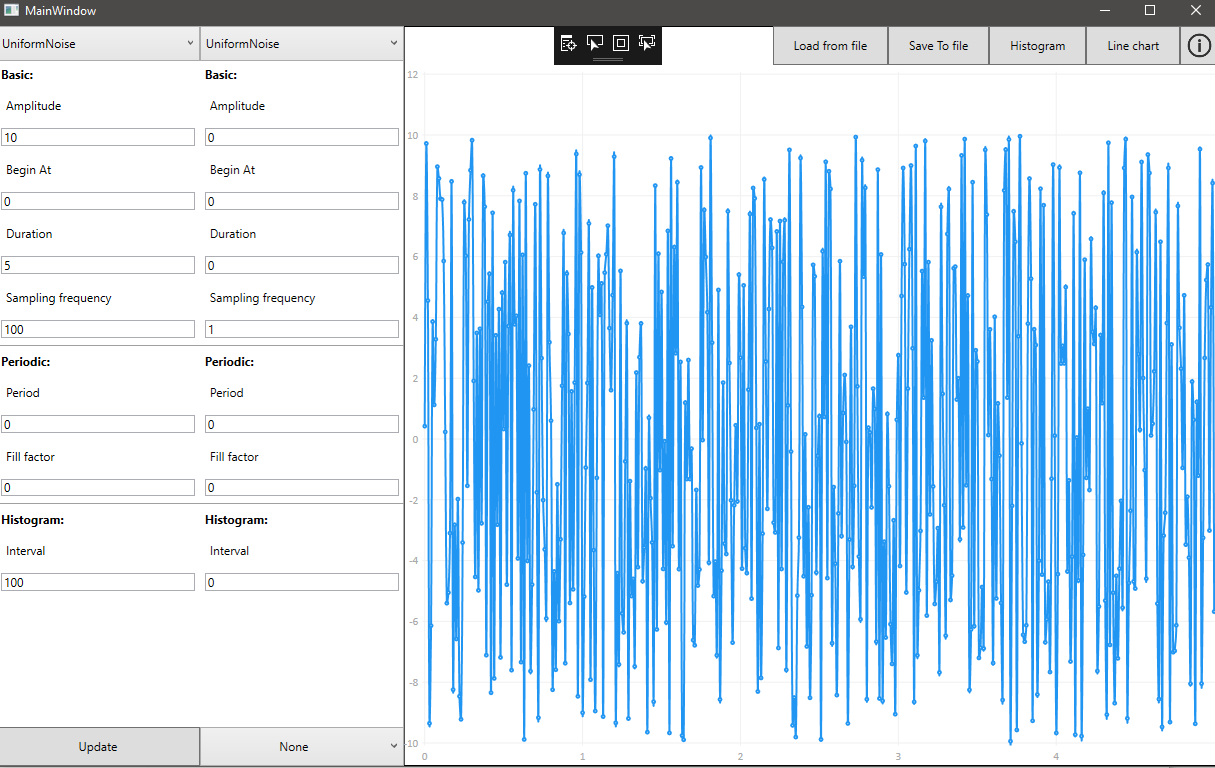
\includegraphics[width=14cm]{images/uni1.PNG}
 \vspace{-0.3cm}
 \caption{Wykres szumu o rozkladzie jednostajnym}
 \label{gui}
\end{figure}

\begin{figure}[H]
 \centering
 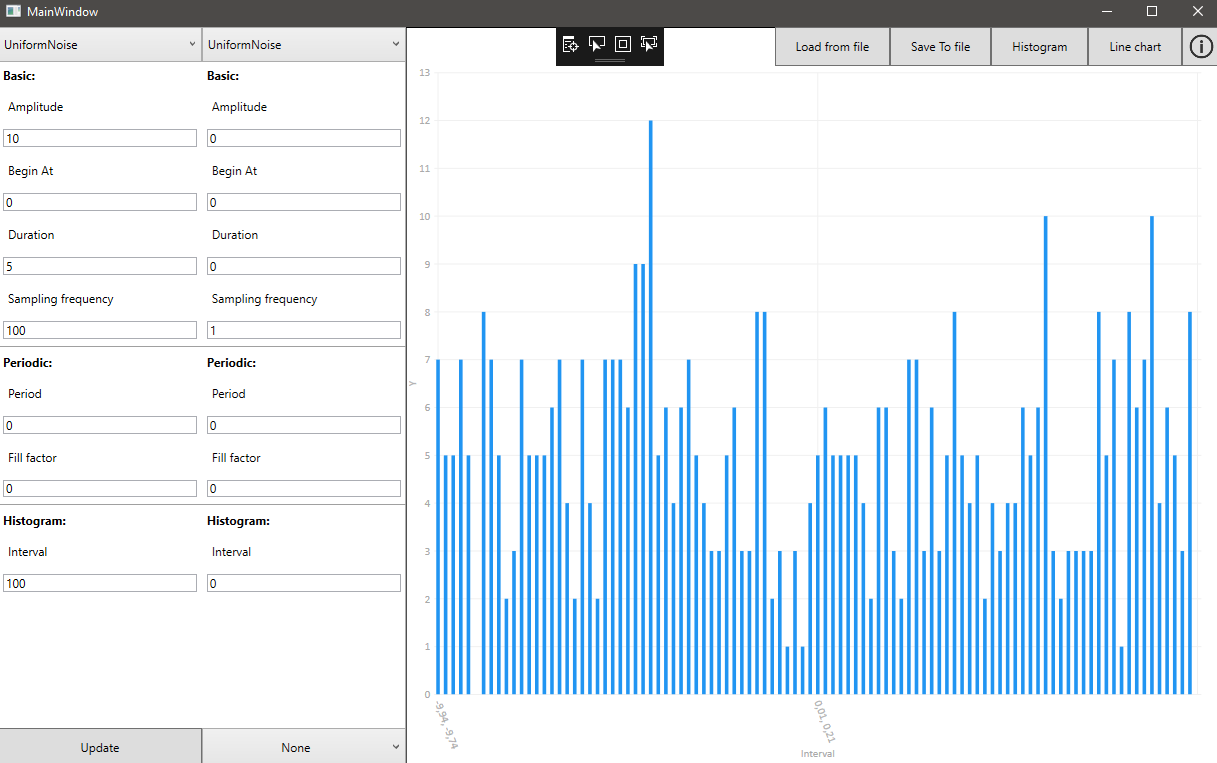
\includegraphics[width=14cm]{images/uni1hist.PNG}
 \vspace{-0.3cm}
 \caption{Histogram dla szumu o rozkladzie jednostajnym}
 \label{gui}
\end{figure}

\begin{figure}[H]
 \centering
 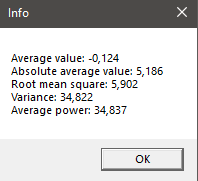
\includegraphics[width=7cm]{images/uni1info.PNG}
 \vspace{-0.3cm}
 \caption{Wyliczone wartosci dla szumu o rozkladzie jednostajnym}
 \label{gui}
\end{figure}

%%%%%%%%%%%%%%%%%%%%%%%%%%%%%%%%%%%%%%%%%%%%%%%%%%%%%%%%%%%%%%%%%%%%%%%%%%%%%%%%%%%%%%%%%%%%%%%%%%%%%%%%%%%%%%%%%
% PODROZDZIAŁ PT. EKSPERYMENT NR 4
%%%%%%%%%%%%%%%%%%%%%%%%%%%%%%%%%%%%%%%%%%%%%%%%%%%%%%%%%%%%%%%%%%%%%%%%%%%%%%%%%%%%%%%%%%%%%%%%%%%%%%%%%%%%%%%%%


\subsection{Eksperyment nr 4 }
\subsubsection{Generowanie skoku jednostkowego}
Celem tego eksperymentu było wygenerowanie skoku jednostkowego.


\subsubsection{Rezultat}

\begin{figure}[H]
 \centering
 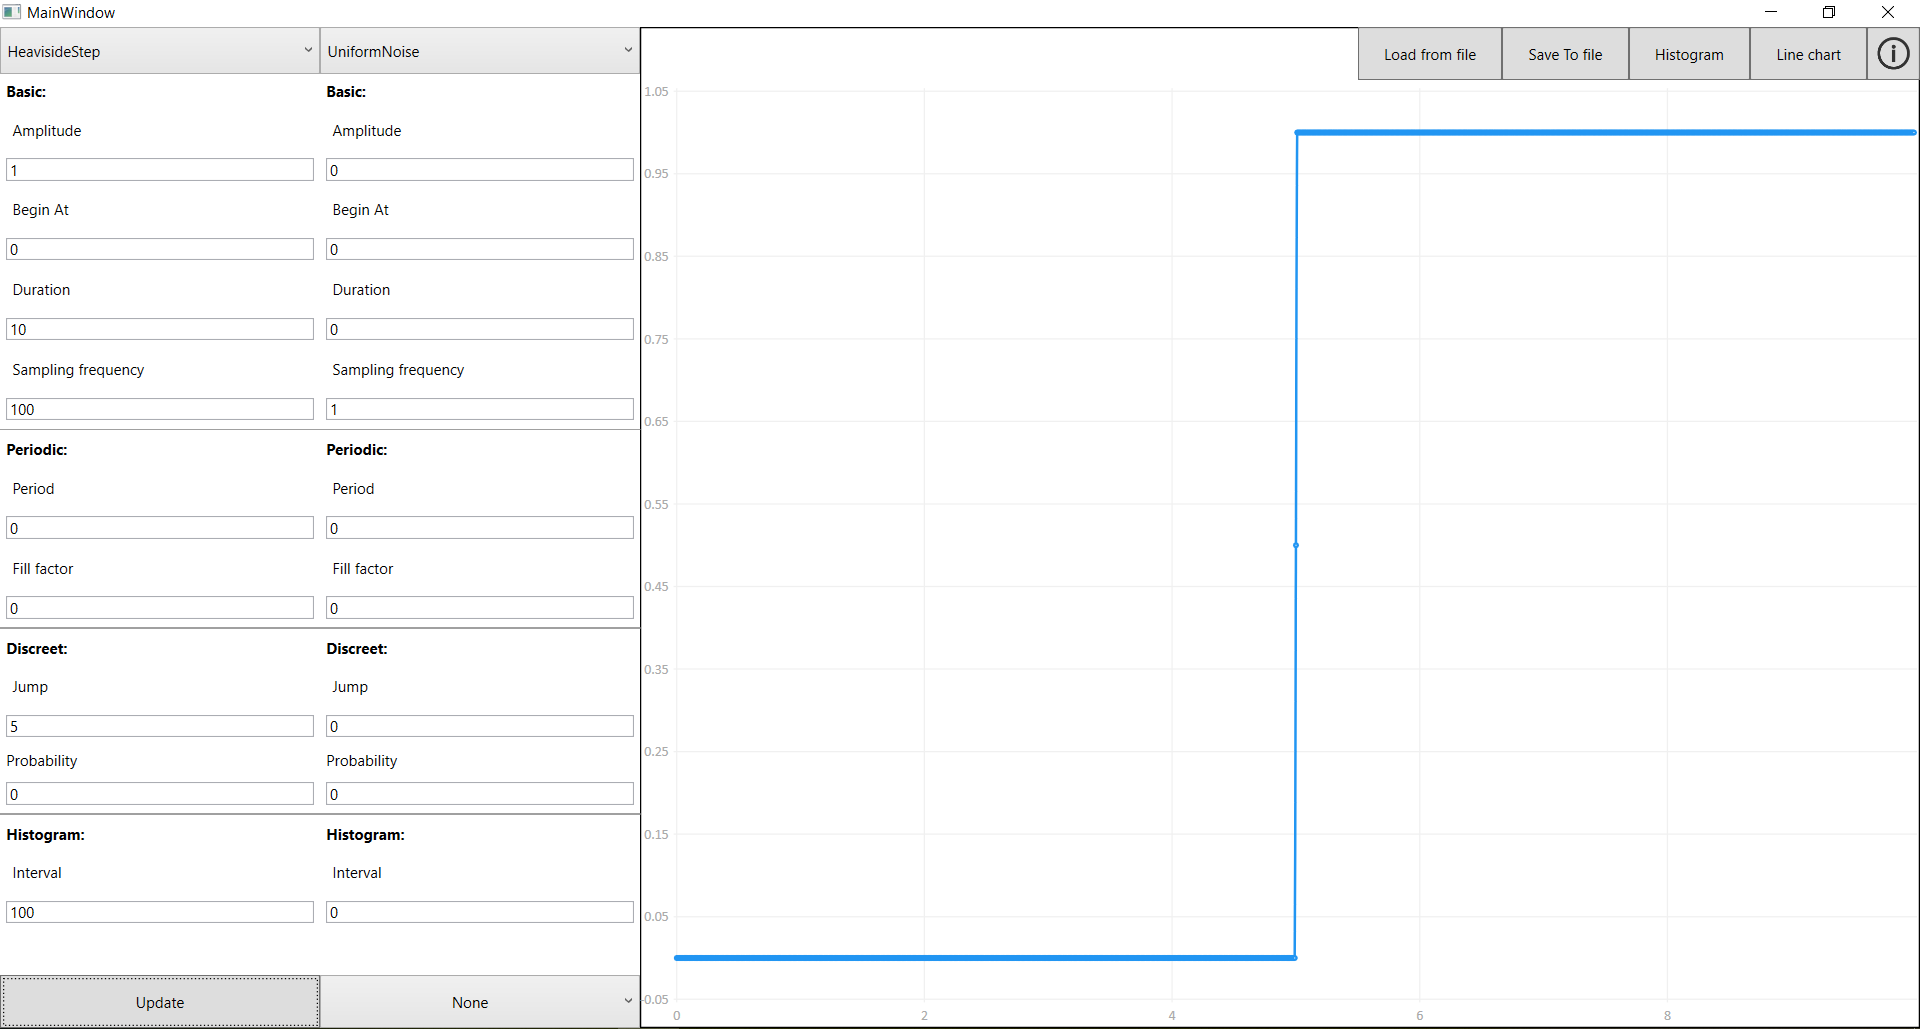
\includegraphics[width=14cm]{images/heav1.PNG}
 \vspace{-0.3cm}
 \caption{Wykres skoku jednostkowego}
 \label{gui}
\end{figure}

\begin{figure}[H]
 \centering
 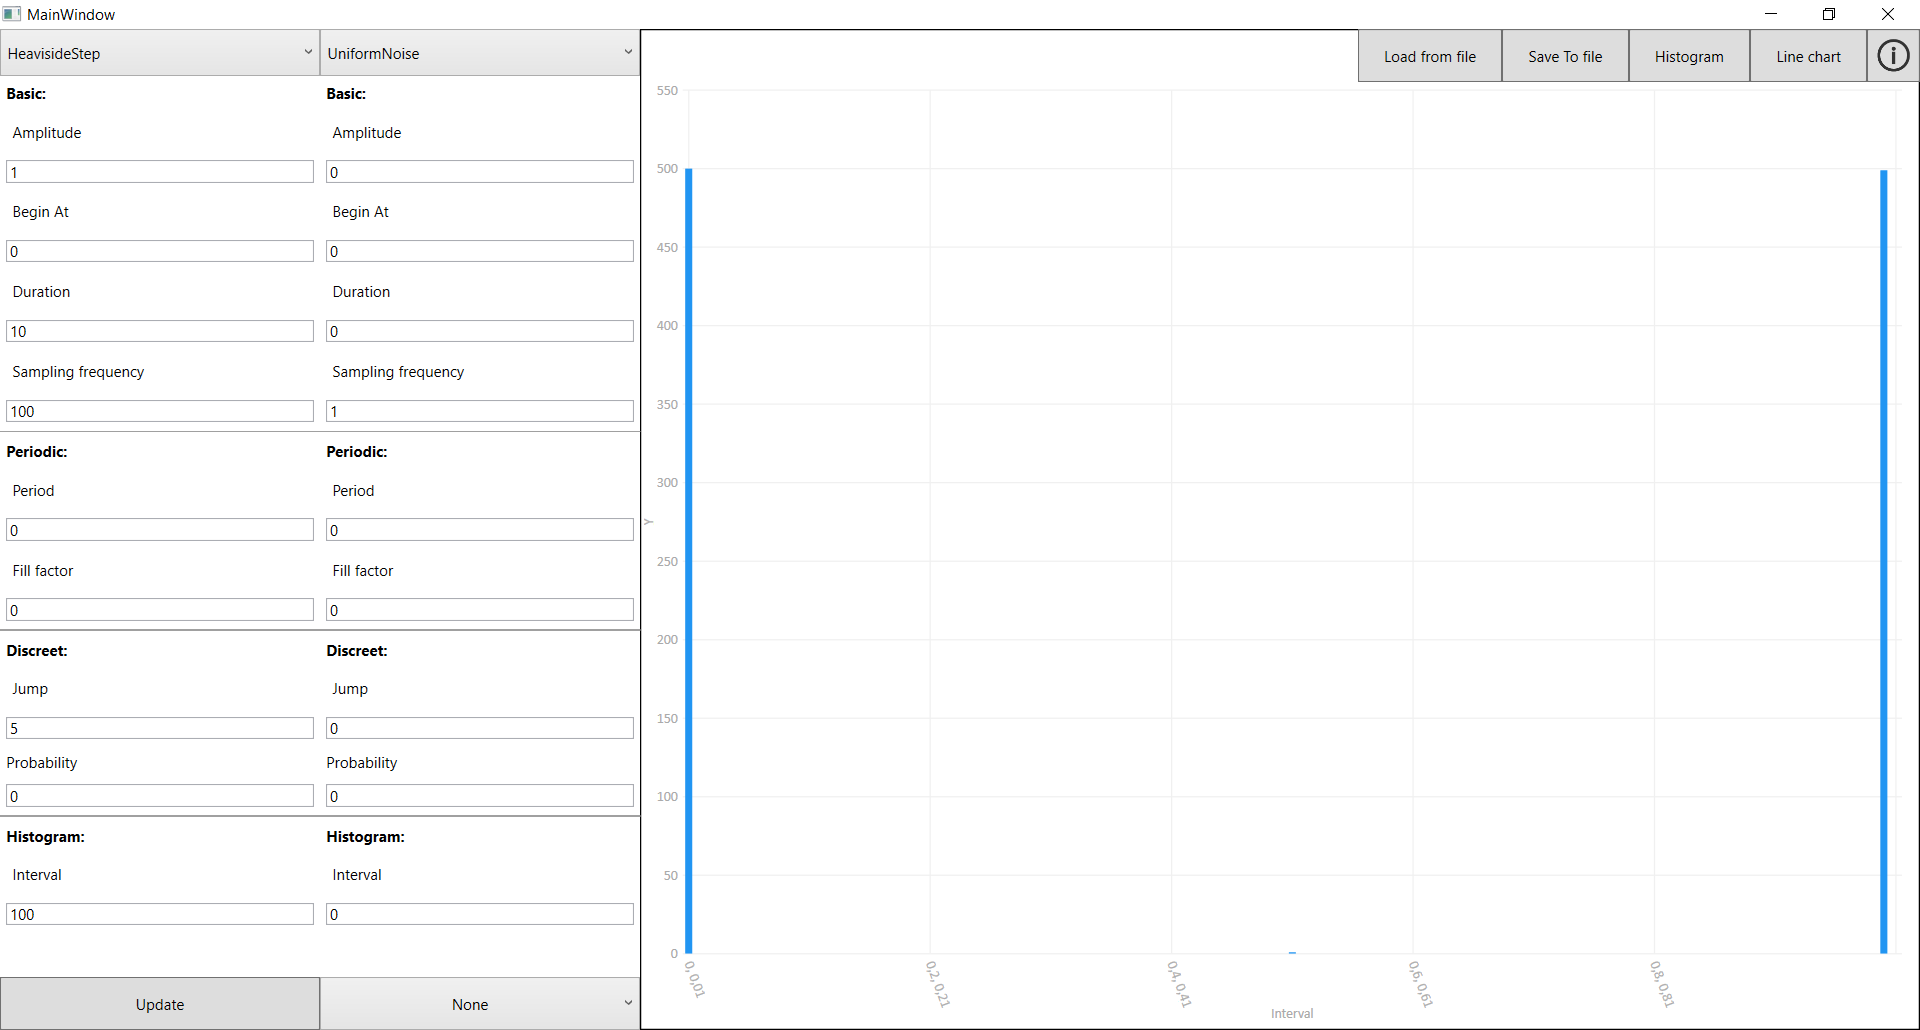
\includegraphics[width=14cm]{images/heav1hist.PNG}
 \vspace{-0.3cm}
 \caption{Histogram dla skoku jednostkowego}
 \label{gui}
\end{figure}

\begin{figure}[H]
 \centering
 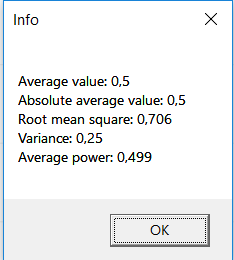
\includegraphics[width=7cm]{images/heav1info.PNG}
 \vspace{-0.3cm}
 \caption{Wyliczone wartosci dla skoku jednostkowego}
 \label{gui}
\end{figure}

%%%%%%%%%%%%%%%%%%%%%%%%%%%%%%%%%%%%%%%%%%%%%%%%%%%%%%%%%%%%%%%%%%%%%%%%%%%%%%%%%%%%%%%%%%%%%%%%%%%%%%%%%%%%%%%%%
% PODROZDZIAŁ PT. EKSPERYMENT NR 5
%%%%%%%%%%%%%%%%%%%%%%%%%%%%%%%%%%%%%%%%%%%%%%%%%%%%%%%%%%%%%%%%%%%%%%%%%%%%%%%%%%%%%%%%%%%%%%%%%%%%%%%%%%%%%%%%%


\subsection{Eksperyment nr 5 }
\subsubsection{Generowanie sygnału sinusoidalnego wyprostowanego jednopołówkowo}
Celem tego eksperymentu było wygenerowanie szumu o rozkladzie jednostajnym.


\subsubsection{Rezultat}

\begin{figure}[H]
 \centering
 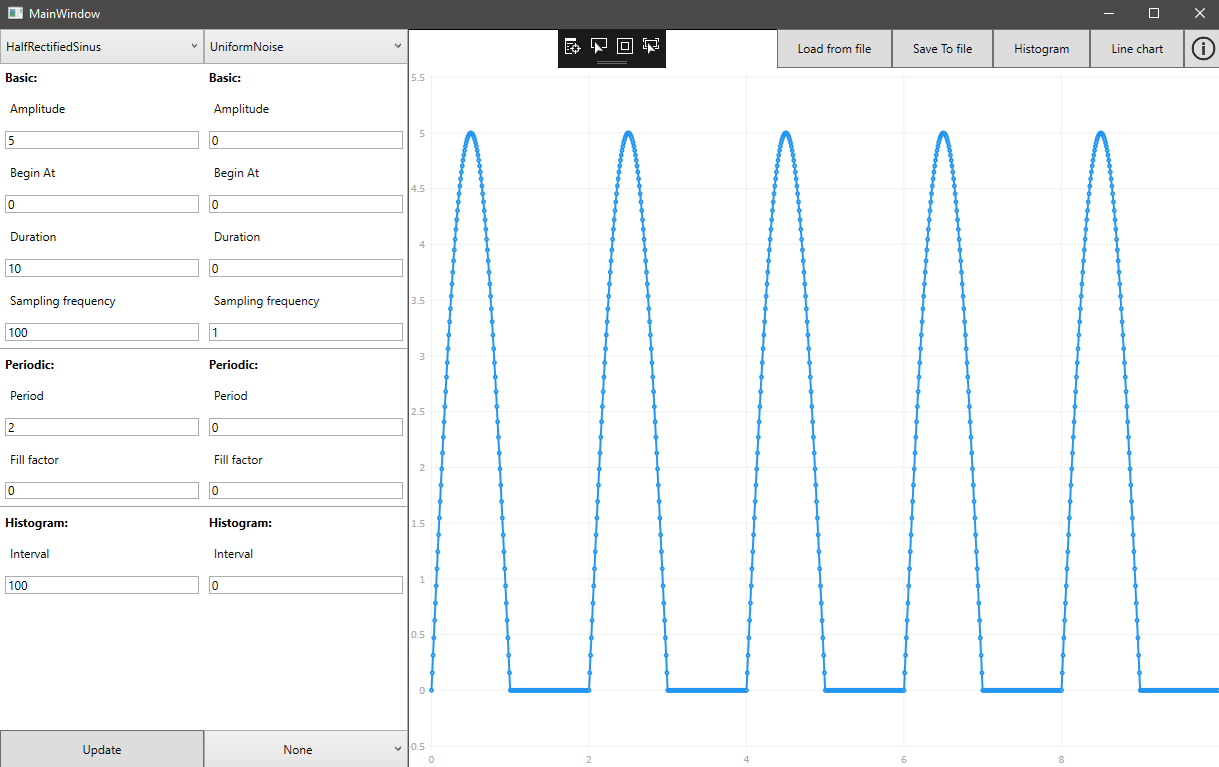
\includegraphics[width=14cm]{images/half1.PNG}
 \vspace{-0.3cm}
 \caption{Wykres sygnału sinusoidalnego wyprostowanego jednopołówkowo}
 \label{gui}
\end{figure}

\begin{figure}[H]
 \centering
 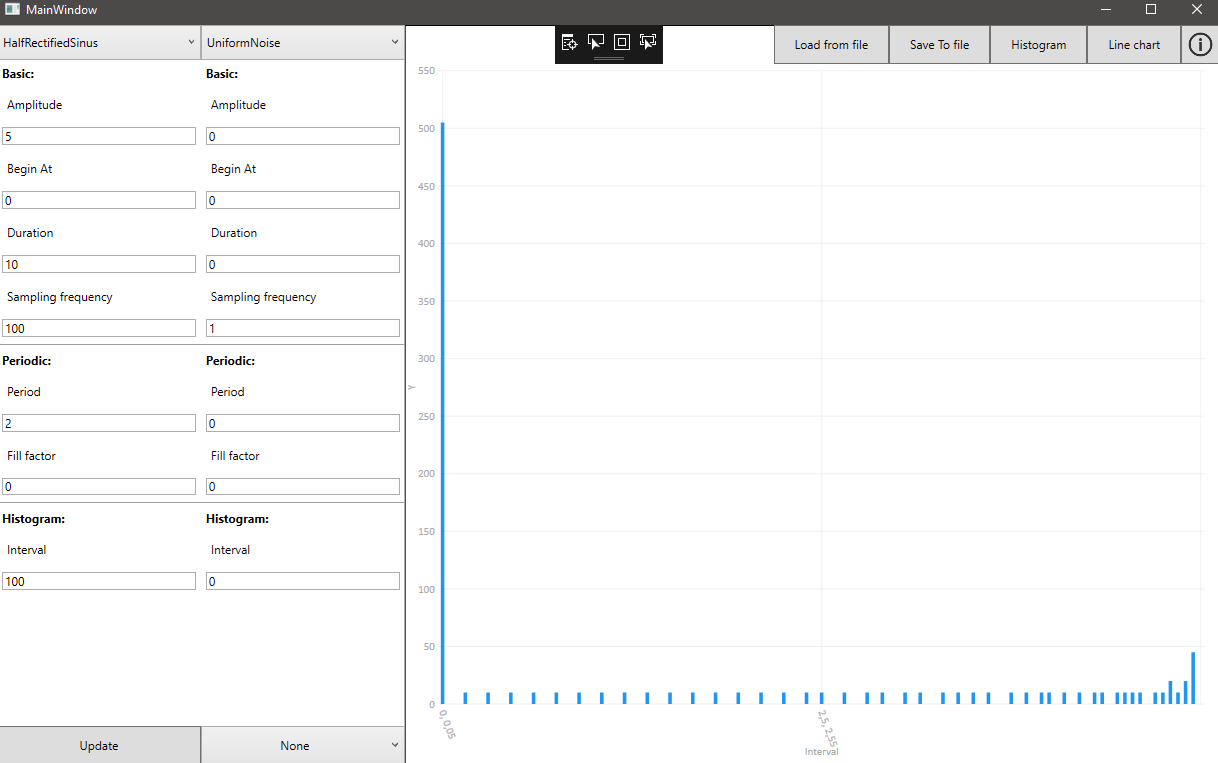
\includegraphics[width=14cm]{images/half1hist.PNG}
 \vspace{-0.3cm}
 \caption{Histogram dlasygnału sinusoidalnego wyprostowanego jednopołówkowo}
 \label{gui}
\end{figure}

\begin{figure}[H]
 \centering
 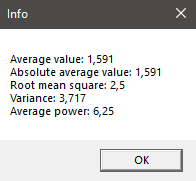
\includegraphics[width=7cm]{images/half1info.PNG}
 \vspace{-0.3cm}
 \caption{Wyliczone wartosci dla sygnału sinusoidalnego wyprostowanego jednopołówkowo}
 \label{gui}
\end{figure}


%%%%%%%%%%%%%%%%%%%%%%%%%%%%%%%%%%%%%%%%%%%%%%%%%%%%%%%%%%%%%%%%%%%%%%%%%%%%%%%%%%%%%%%%%%%%%%%%%%%%%%%%%%%%%%%%%
% PODROZDZIAŁ PT. EKSPERYMENT NR 6
%%%%%%%%%%%%%%%%%%%%%%%%%%%%%%%%%%%%%%%%%%%%%%%%%%%%%%%%%%%%%%%%%%%%%%%%%%%%%%%%%%%%%%%%%%%%%%%%%%%%%%%%%%%%%%%%%


\subsection{Eksperyment nr 6 }
\subsubsection{Generowanie sygnału sinusoidalnego wyprostowanego dwupołówkowo}
Celem tego eksperymentu było wygenerowanie sygnału sinusoidalnego wyprostowanego dwupołówkowo.

\subsubsection{Rezultat}

\begin{figure}[H]
 \centering
 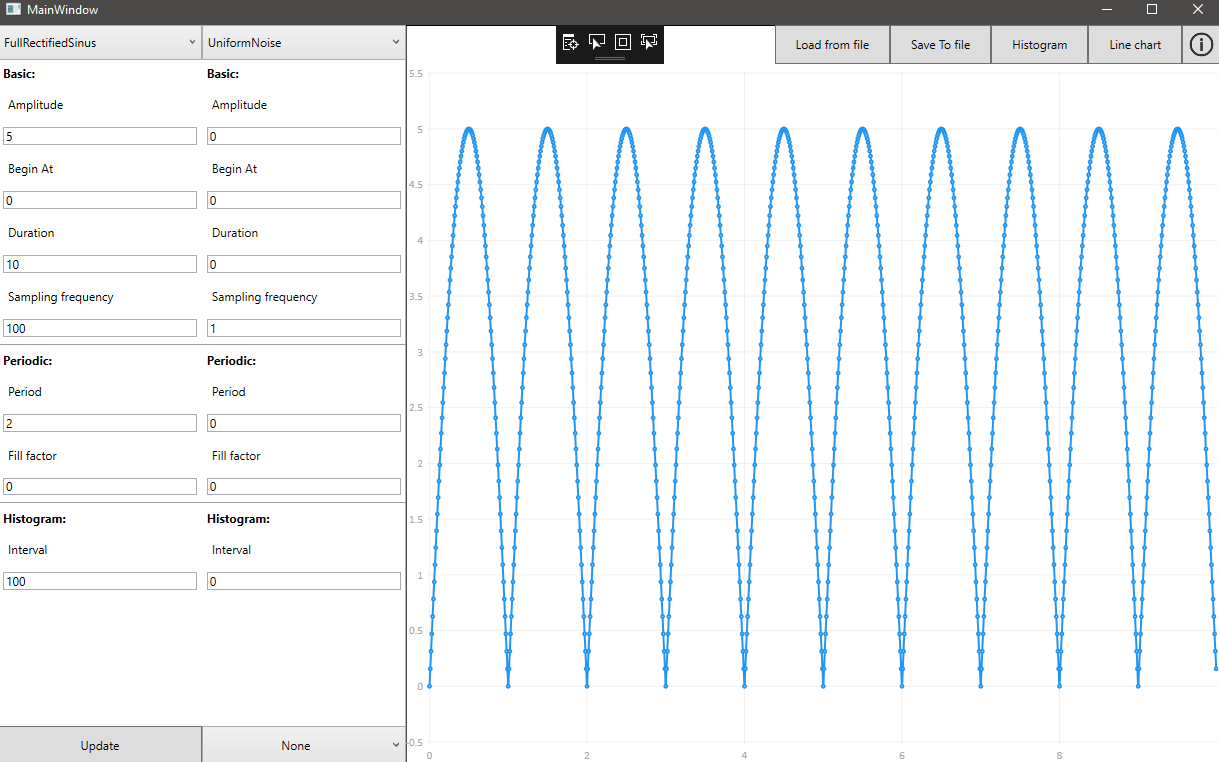
\includegraphics[width=14cm]{images/full1.PNG}
 \vspace{-0.3cm}
 \caption{Wykres sygnału sinusoidalnego wyprostowanego dwupołówkowo}
 \label{gui}
\end{figure}

\begin{figure}[H]
 \centering
 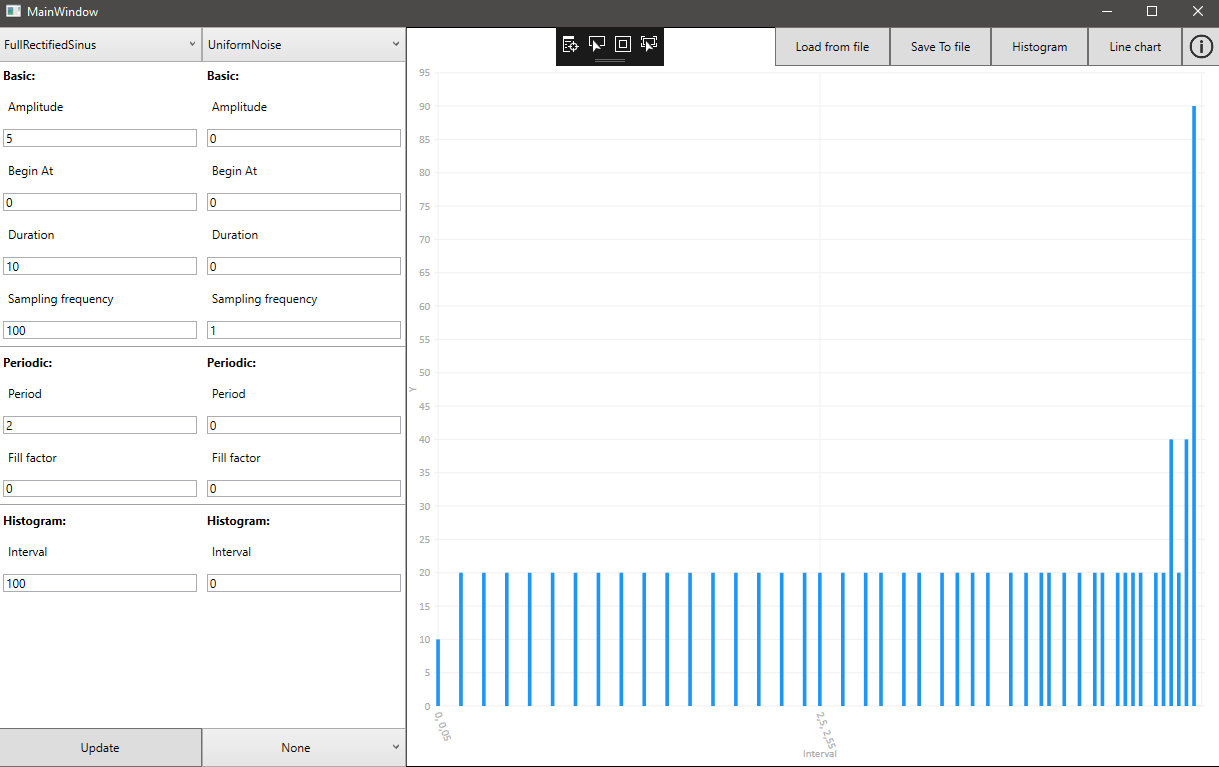
\includegraphics[width=14cm]{images/full1hist.PNG}
 \vspace{-0.3cm}
 \caption{Histogram dla sygnału sinusoidalnego wyprostowanego dwupołówkowo}
 \label{gui}
\end{figure}

\begin{figure}[H]
 \centering
 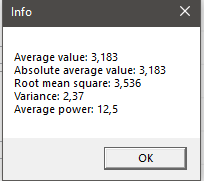
\includegraphics[width=7cm]{images/full1info.PNG}
 \vspace{-0.3cm}
 \caption{Wyliczone wartosci dla sygnału sinusoidalnego wyprostowanego dwupołówkowo}
 \label{gui}
\end{figure}


%%%%%%%%%%%%%%%%%%%%%%%%%%%%%%%%%%%%%%%%%%%%%%%%%%%%%%%%%%%%%%%%%%%%%%%%%%%%%%%%%%%%%%%%%%%%%%%%%%%%%%%%%%%%%%%%%
% PODROZDZIAŁ PT. EKSPERYMENT NR 7
%%%%%%%%%%%%%%%%%%%%%%%%%%%%%%%%%%%%%%%%%%%%%%%%%%%%%%%%%%%%%%%%%%%%%%%%%%%%%%%%%%%%%%%%%%%%%%%%%%%%%%%%%%%%%%%%%


\subsection{Eksperyment nr 7 }
\subsubsection{Generowanie sygnału protokątnego}
Celem tego eksperymentu było wygenerowanie sygnału protokątnego.


\subsubsection{Rezultat}

\begin{figure}[H]
 \centering
 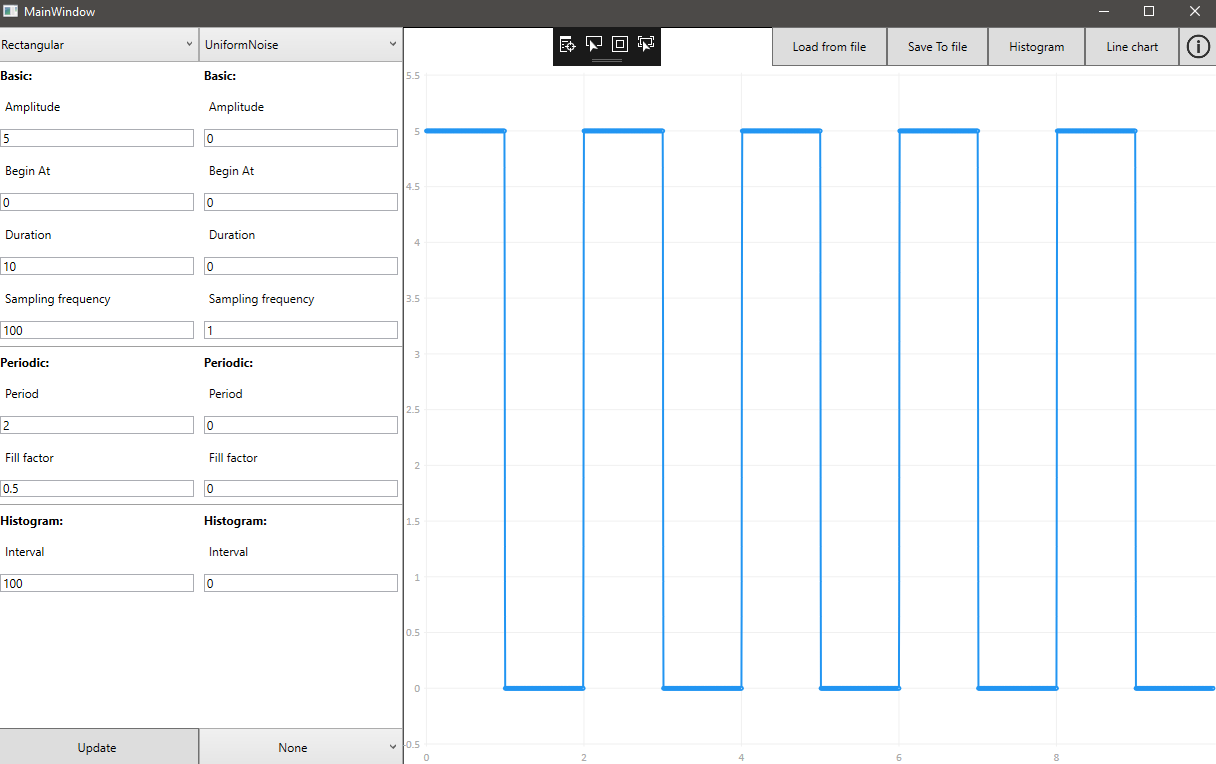
\includegraphics[width=14cm]{images/rect1.PNG}
 \vspace{-0.3cm}
 \caption{Wykres sygnału protokątnego}
 \label{gui}
\end{figure}

\begin{figure}[H]
 \centering
 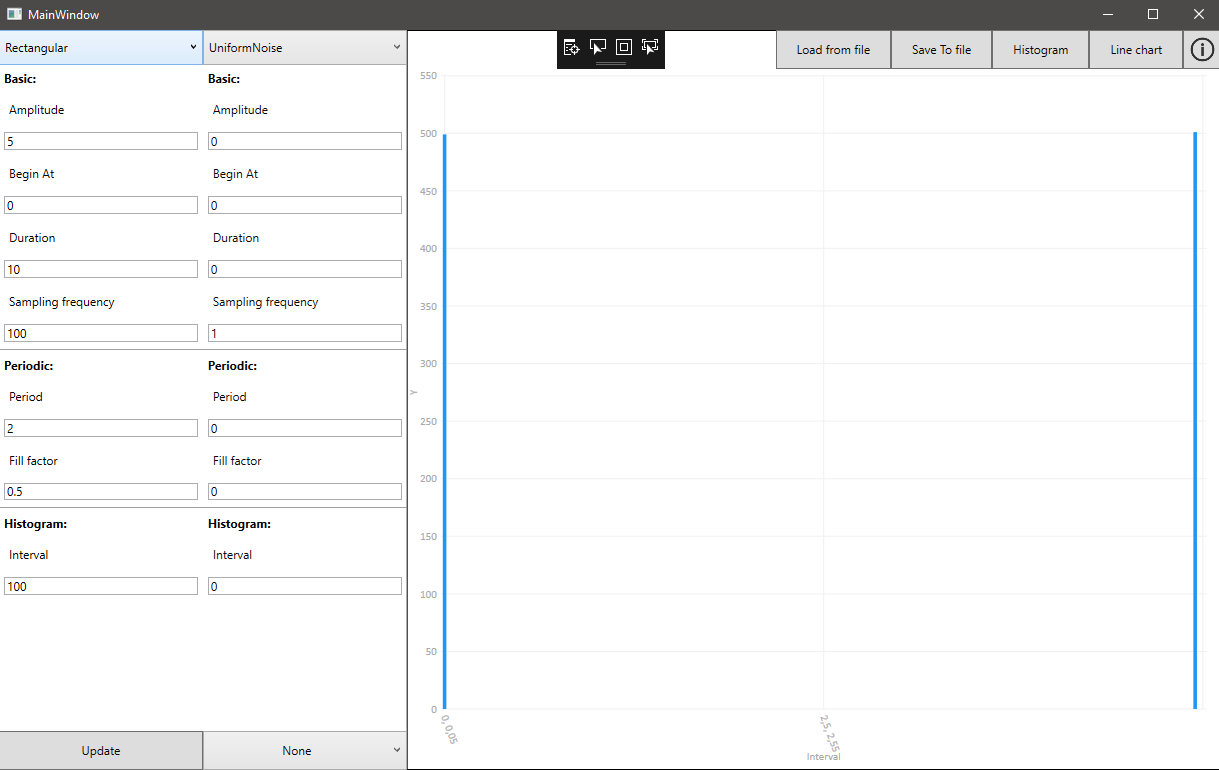
\includegraphics[width=14cm]{images/rect1hist.PNG}
 \vspace{-0.3cm}
 \caption{Histogram dla sygnału protokątnego}
 \label{gui}
\end{figure}

\begin{figure}[H]
 \centering
 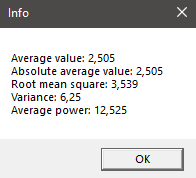
\includegraphics[width=7cm]{images/rect1info.PNG}
 \vspace{-0.3cm}
 \caption{Wyliczone wartosci dla sygnału protokątnego}
 \label{gui}
\end{figure}


%%%%%%%%%%%%%%%%%%%%%%%%%%%%%%%%%%%%%%%%%%%%%%%%%%%%%%%%%%%%%%%%%%%%%%%%%%%%%%%%%%%%%%%%%%%%%%%%%%%%%%%%%%%%%%%%%
% PODROZDZIAŁ PT. EKSPERYMENT NR 8
%%%%%%%%%%%%%%%%%%%%%%%%%%%%%%%%%%%%%%%%%%%%%%%%%%%%%%%%%%%%%%%%%%%%%%%%%%%%%%%%%%%%%%%%%%%%%%%%%%%%%%%%%%%%%%%%%


\subsection{Eksperyment nr 8 }
\subsubsection{Generowanie sygnału protokątnego symetrycznego}
Celem tego eksperymentu było wygenerowanie sygnału protokątnego symetrycznego.


\subsubsection{Rezultat}

\begin{figure}[H]
 \centering
 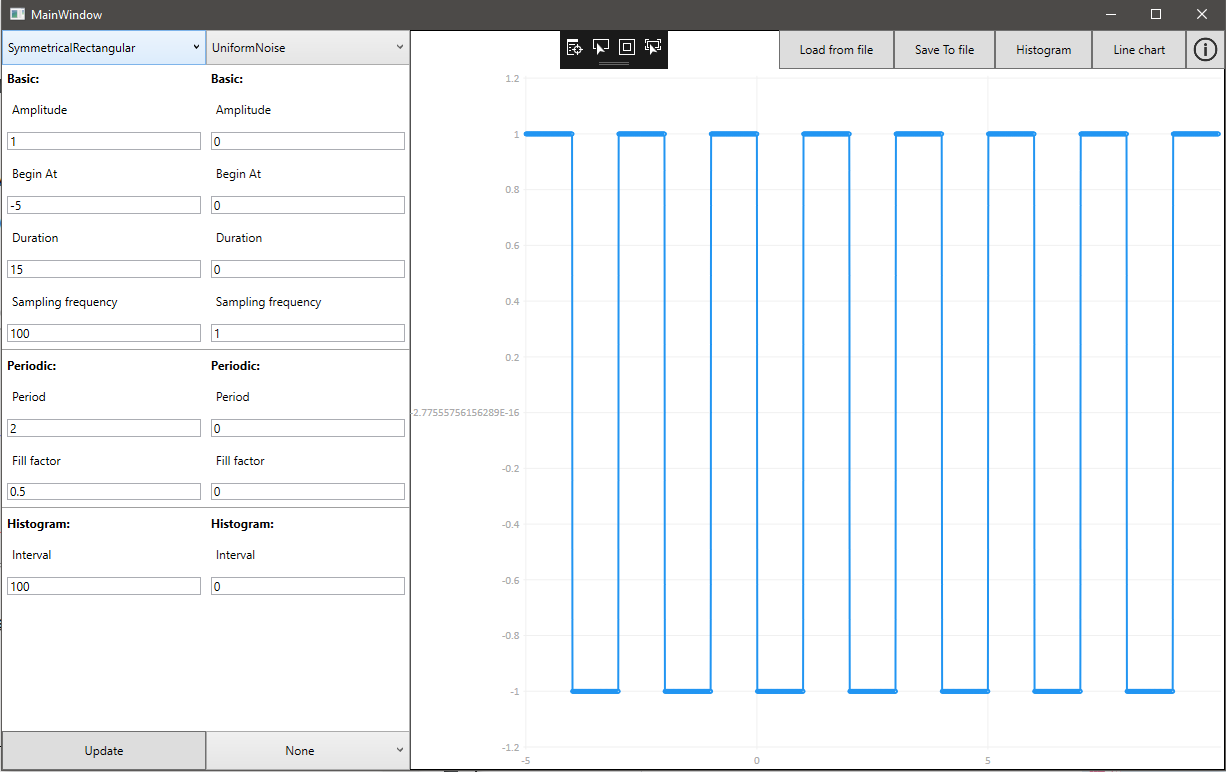
\includegraphics[width=14cm]{images/symrect1.PNG}
 \vspace{-0.3cm}
 \caption{Wykres sygnału protokątnego symetrycznego}
 \label{gui}
\end{figure}

\begin{figure}[H]
 \centering
 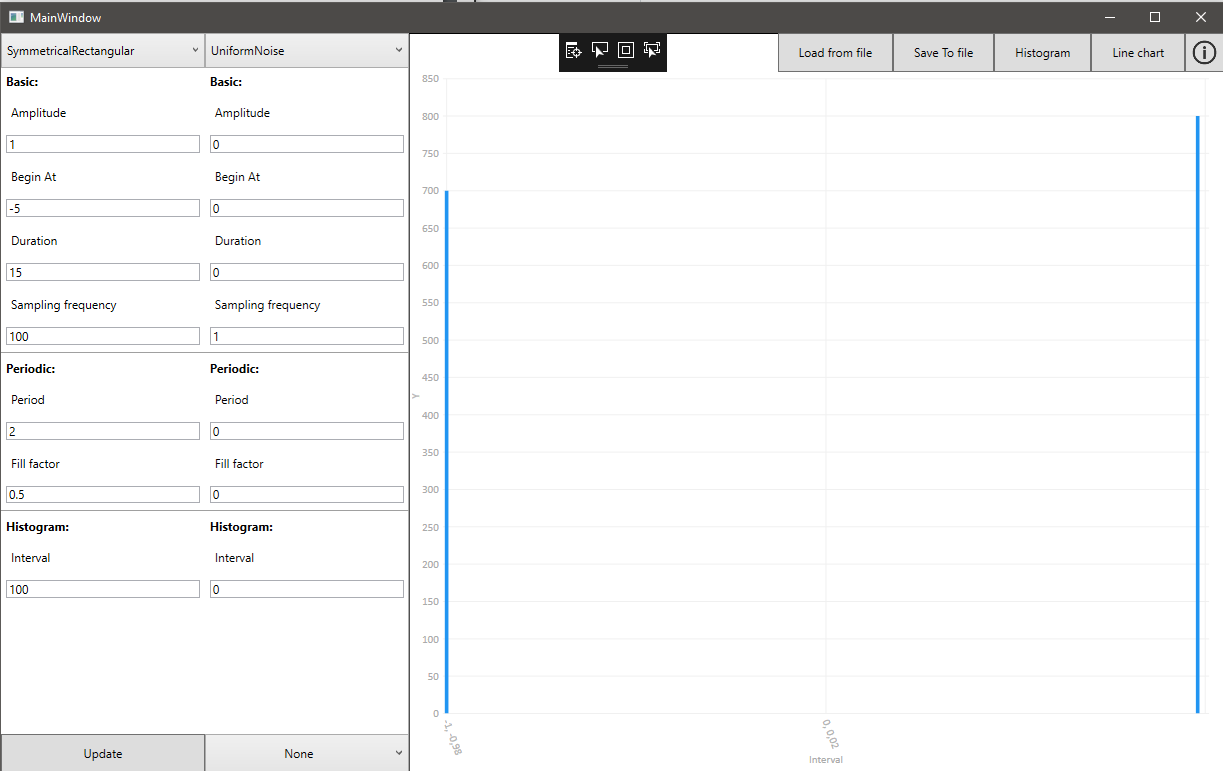
\includegraphics[width=14cm]{images/symrect1hist.PNG}
 \vspace{-0.3cm}
 \caption{Histogram dla sygnału protokątnego symetrycznego}
 \label{gui}
\end{figure}

\begin{figure}[H]
 \centering
 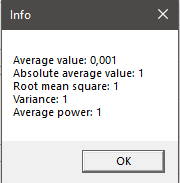
\includegraphics[width=7cm]{images/symrect1info.PNG}
 \vspace{-0.3cm}
 \caption{Wyliczone wartosci dla sygnału protokątnego symetrycznego}
 \label{gui}
\end{figure}

%%%%%%%%%%%%%%%%%%%%%%%%%%%%%%%%%%%%%%%%%%%%%%%%%%%%%%%%%%%%%%%%%%%%%%%%%%%%%%%%%%%%%%%%%%%%%%%%%%%%%%%%%%%%%%%%%
% PODROZDZIAŁ PT. EKSPERYMENT NR 9
%%%%%%%%%%%%%%%%%%%%%%%%%%%%%%%%%%%%%%%%%%%%%%%%%%%%%%%%%%%%%%%%%%%%%%%%%%%%%%%%%%%%%%%%%%%%%%%%%%%%%%%%%%%%%%%%%


\subsection{Eksperyment nr 9 }
\subsubsection{Generowanie sygnału trójkątnego}
Celem tego eksperymentu było wygenerowanie sygnału trójkątnego.


\subsubsection{Rezultat}

\begin{figure}[H]
 \centering
 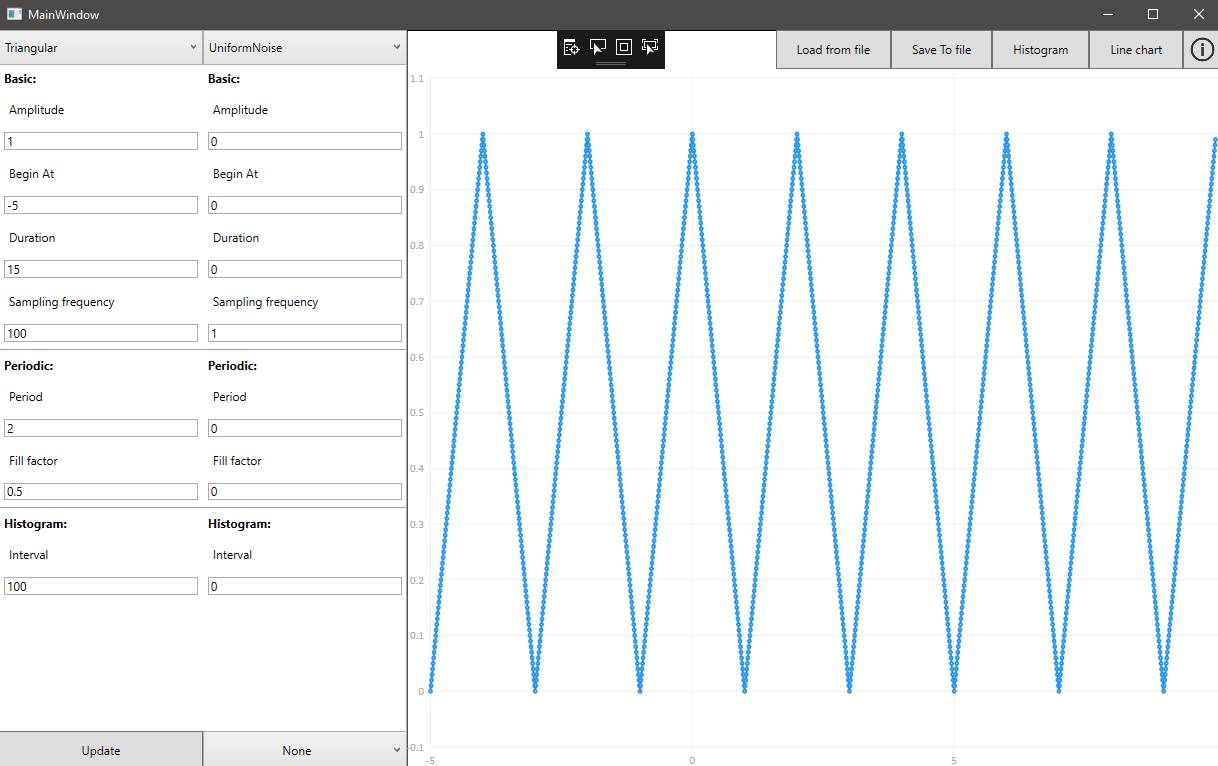
\includegraphics[width=14cm]{images/trian1.PNG}
 \vspace{-0.3cm}
 \caption{Wykres sygnału trójkątnego}
 \label{gui}
\end{figure}

\begin{figure}[H]
 \centering
 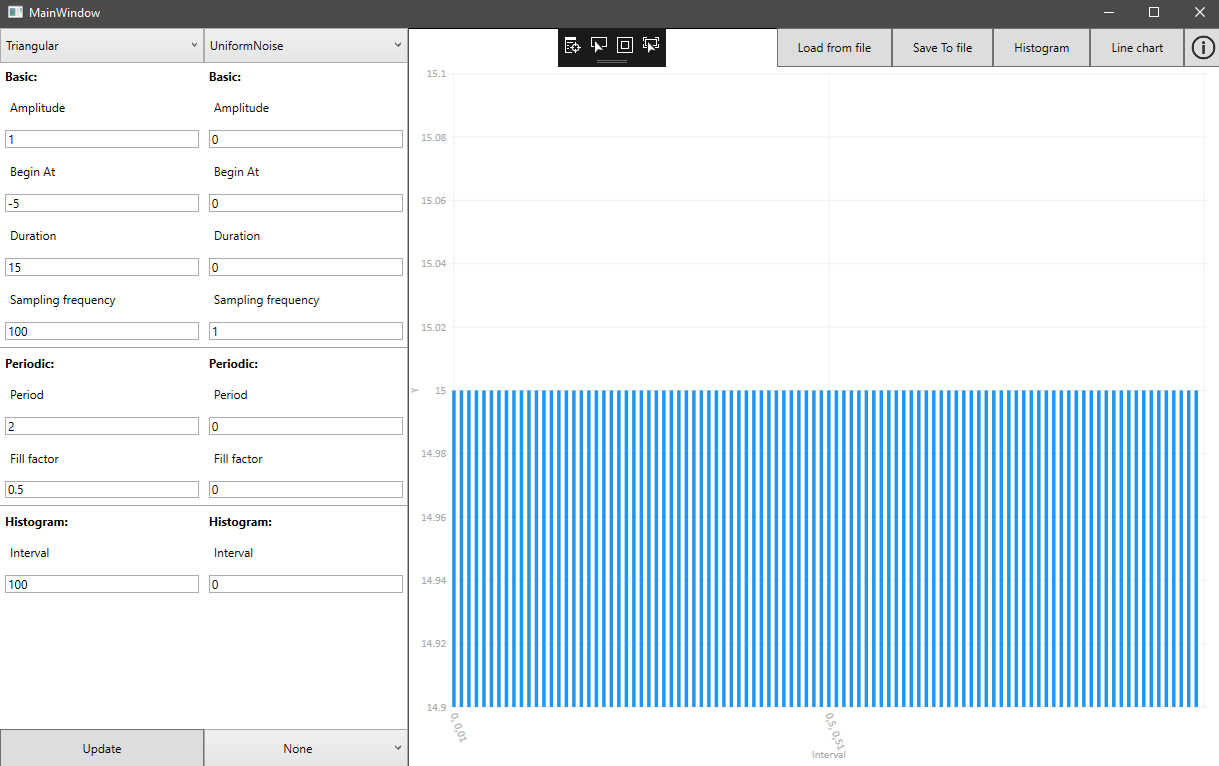
\includegraphics[width=14cm]{images/trian1hist.PNG}
 \vspace{-0.3cm}
 \caption{Histogram dla sygnału trójkątnego}
 \label{gui}
\end{figure}

\begin{figure}[H]
 \centering
 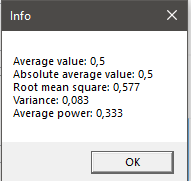
\includegraphics[width=7cm]{images/trian1info.PNG}
 \vspace{-0.3cm}
 \caption{Wyliczone wartosci dla sygnału trójkątnego}
 \label{gui}
\end{figure}

%%%%%%%%%%%%%%%%%%%%%%%%%%%%%%%%%%%%
% PODROZDZIAŁ PT. EKSPERYMENT NR 10
%%%%%%%%%%%%%%%%%%%%%%%%%%%%%%%%%%%%%%%%%%%%%%%%%%%%%%%%%%%%%%%%%%%%%%%%%%%%%%%%%%%%%%%%%%%%%%%%%%%%%%%%%%%%%%%%%


\subsection{Eksperyment nr 10 }
\subsubsection{Generowanie impulsu jednostkowego (delty Kroneckera) }
Celem tego eksperymentu było wygenerowanie impulsu jednostkowego.


\subsubsection{Rezultat}

\begin{figure}[H]
 \centering
 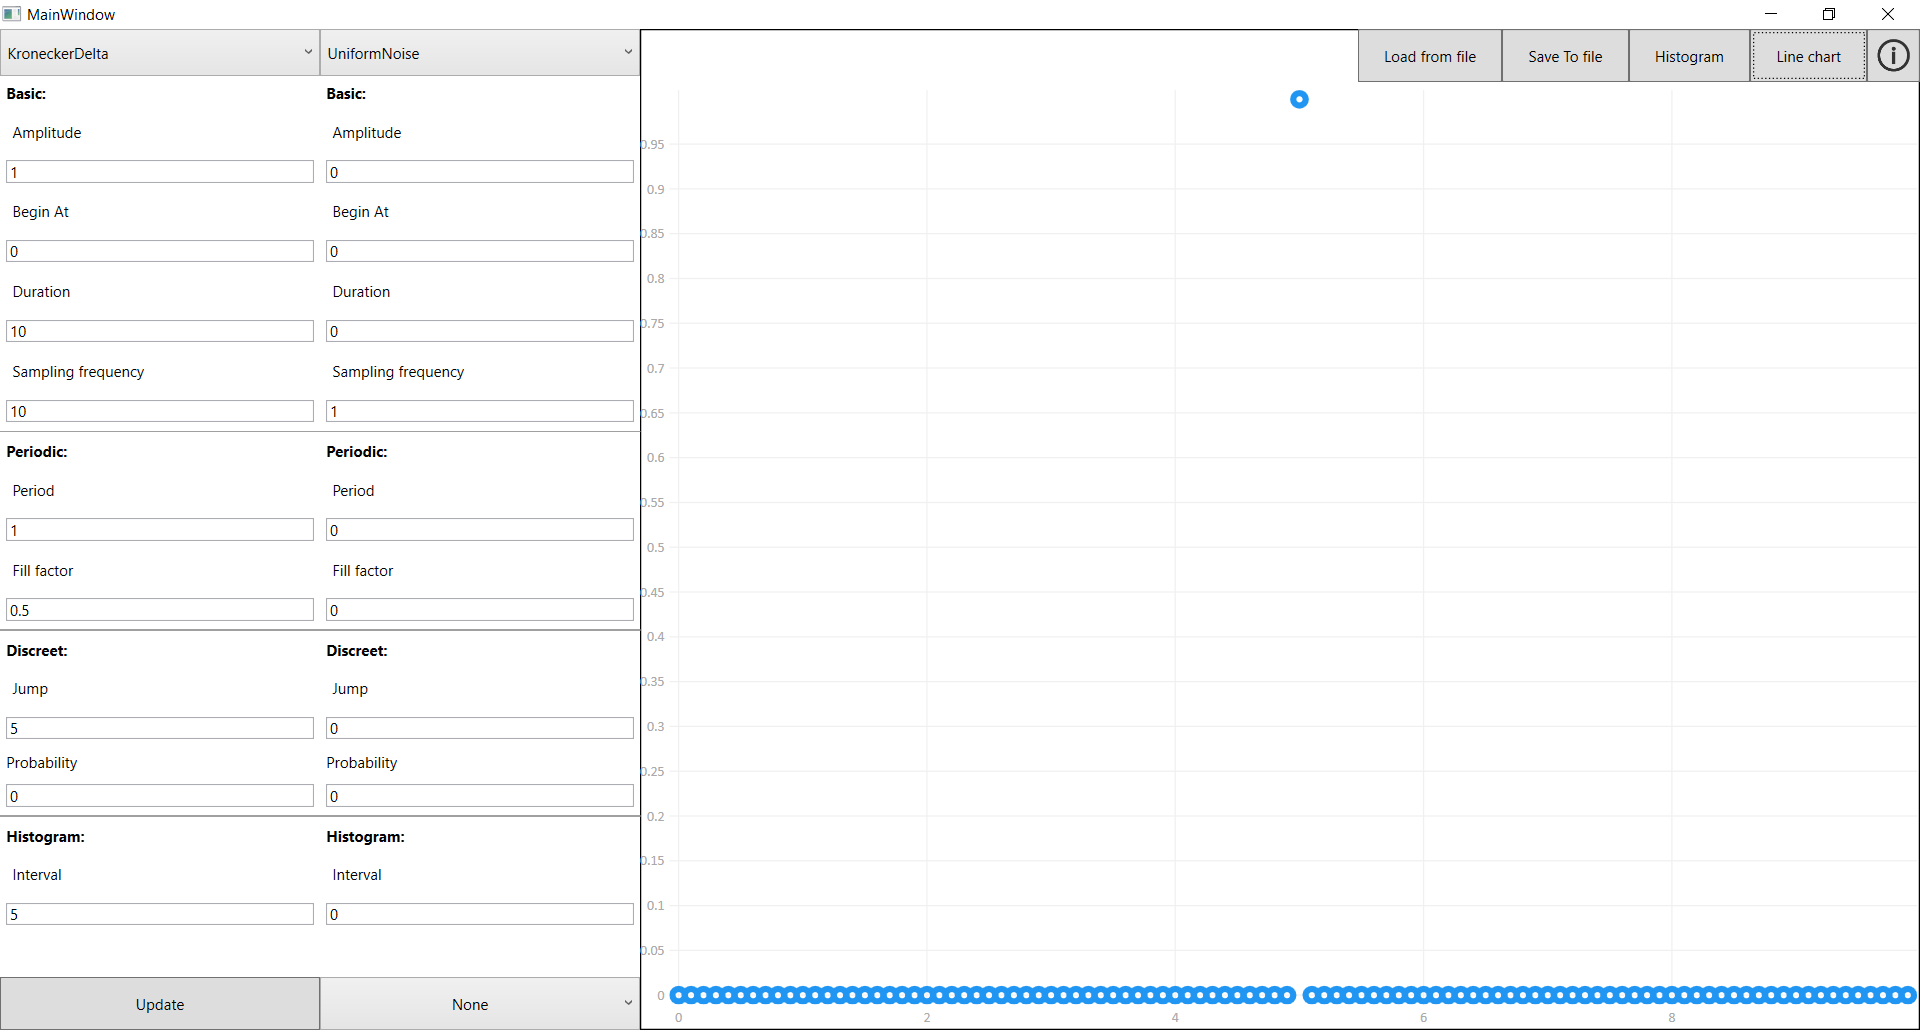
\includegraphics[width=14cm]{images/kron1.PNG}
 \vspace{-0.3cm}
 \caption{Wykres impulsu jednostkowego}
 \label{gui}
\end{figure}

\begin{figure}[H]
 \centering
 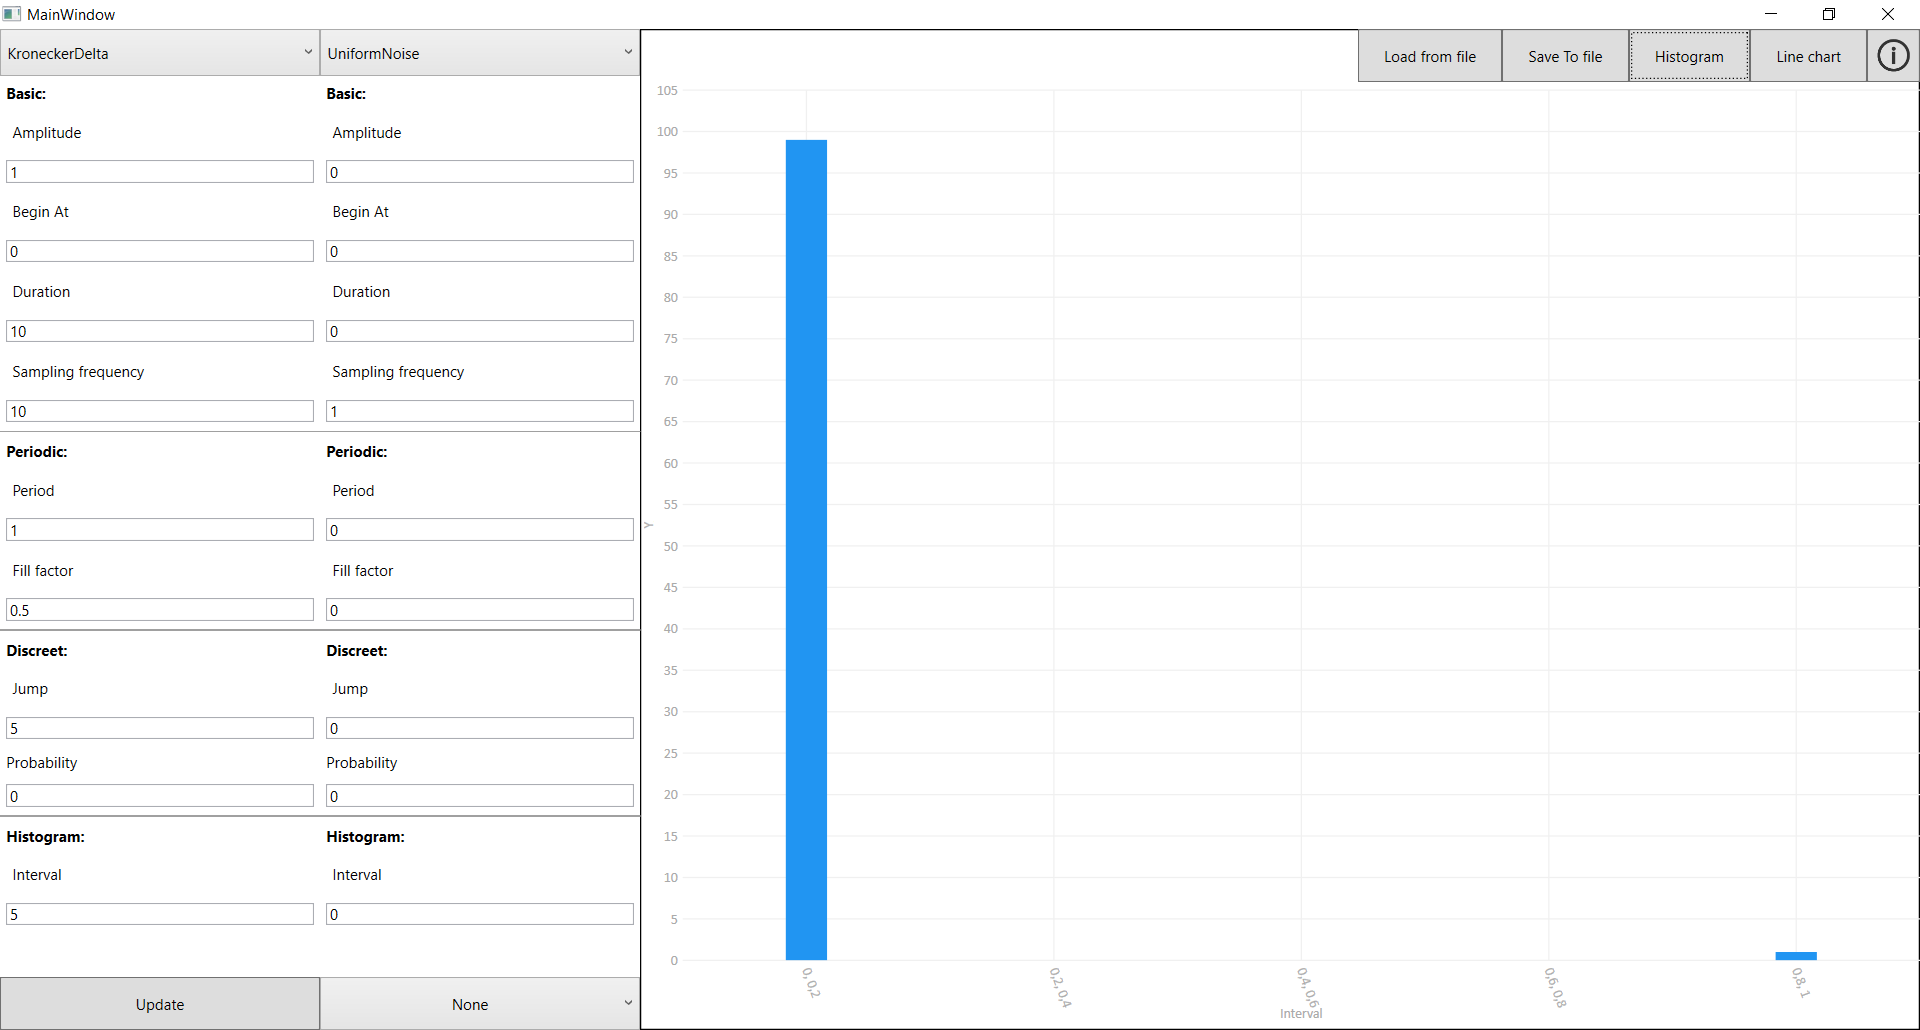
\includegraphics[width=14cm]{images/kron1hist.PNG}
 \vspace{-0.3cm}
 \caption{Histogram dla impulsu jednostkowego}
 \label{gui}
\end{figure}

\begin{figure}[H]
 \centering
 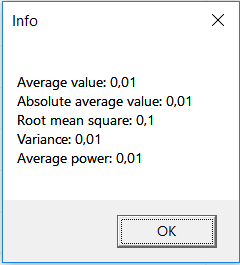
\includegraphics[width=7cm]{images/kron1info.PNG}
 \vspace{-0.3cm}
 \caption{Wyliczone wartosci dla impulsu jednostkowego}
 \label{gui}
\end{figure}

%%%%%%%%%%%%%%%%%%%%%%%%%%%%%%%%%%%%
% PODROZDZIAŁ PT. EKSPERYMENT NR 11
%%%%%%%%%%%%%%%%%%%%%%%%%%%%%%%%%%%%%%%%%%%%%%%%%%%%%%%%%%%%%%%%%%%%%%%%%%%%%%%%%%%%%%%%%%%%%%%%%%%%%%%%%%%%%%%%%


\subsection{Eksperyment nr 11 }
\subsubsection{Generowanie szumu impulsowego}
Celem tego eksperymentu było wygenerowanie szumu impulsowego.


\subsubsection{Rezultat}

\begin{figure}[H]
 \centering
 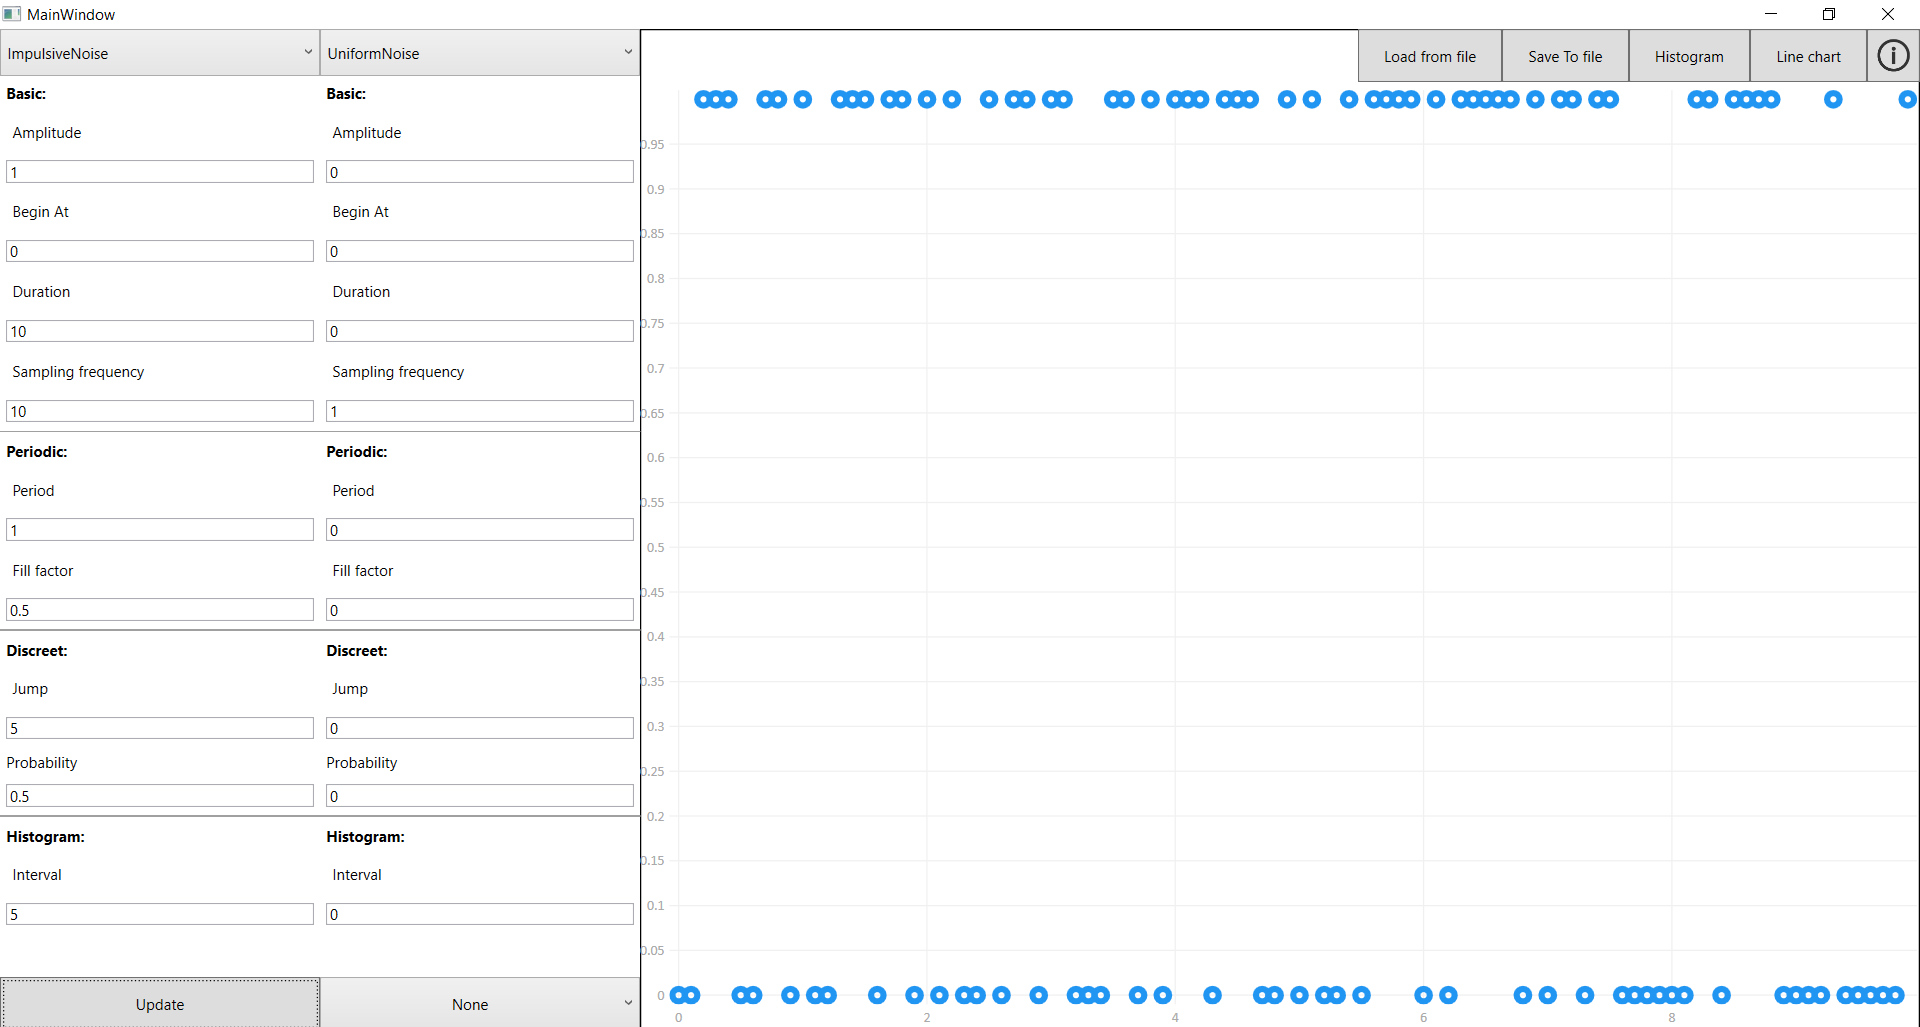
\includegraphics[width=14cm]{images/imp1.PNG}
 \vspace{-0.3cm}
 \caption{Wykres szumu impulsowego}
 \label{gui}
\end{figure}

\begin{figure}[H]
 \centering
 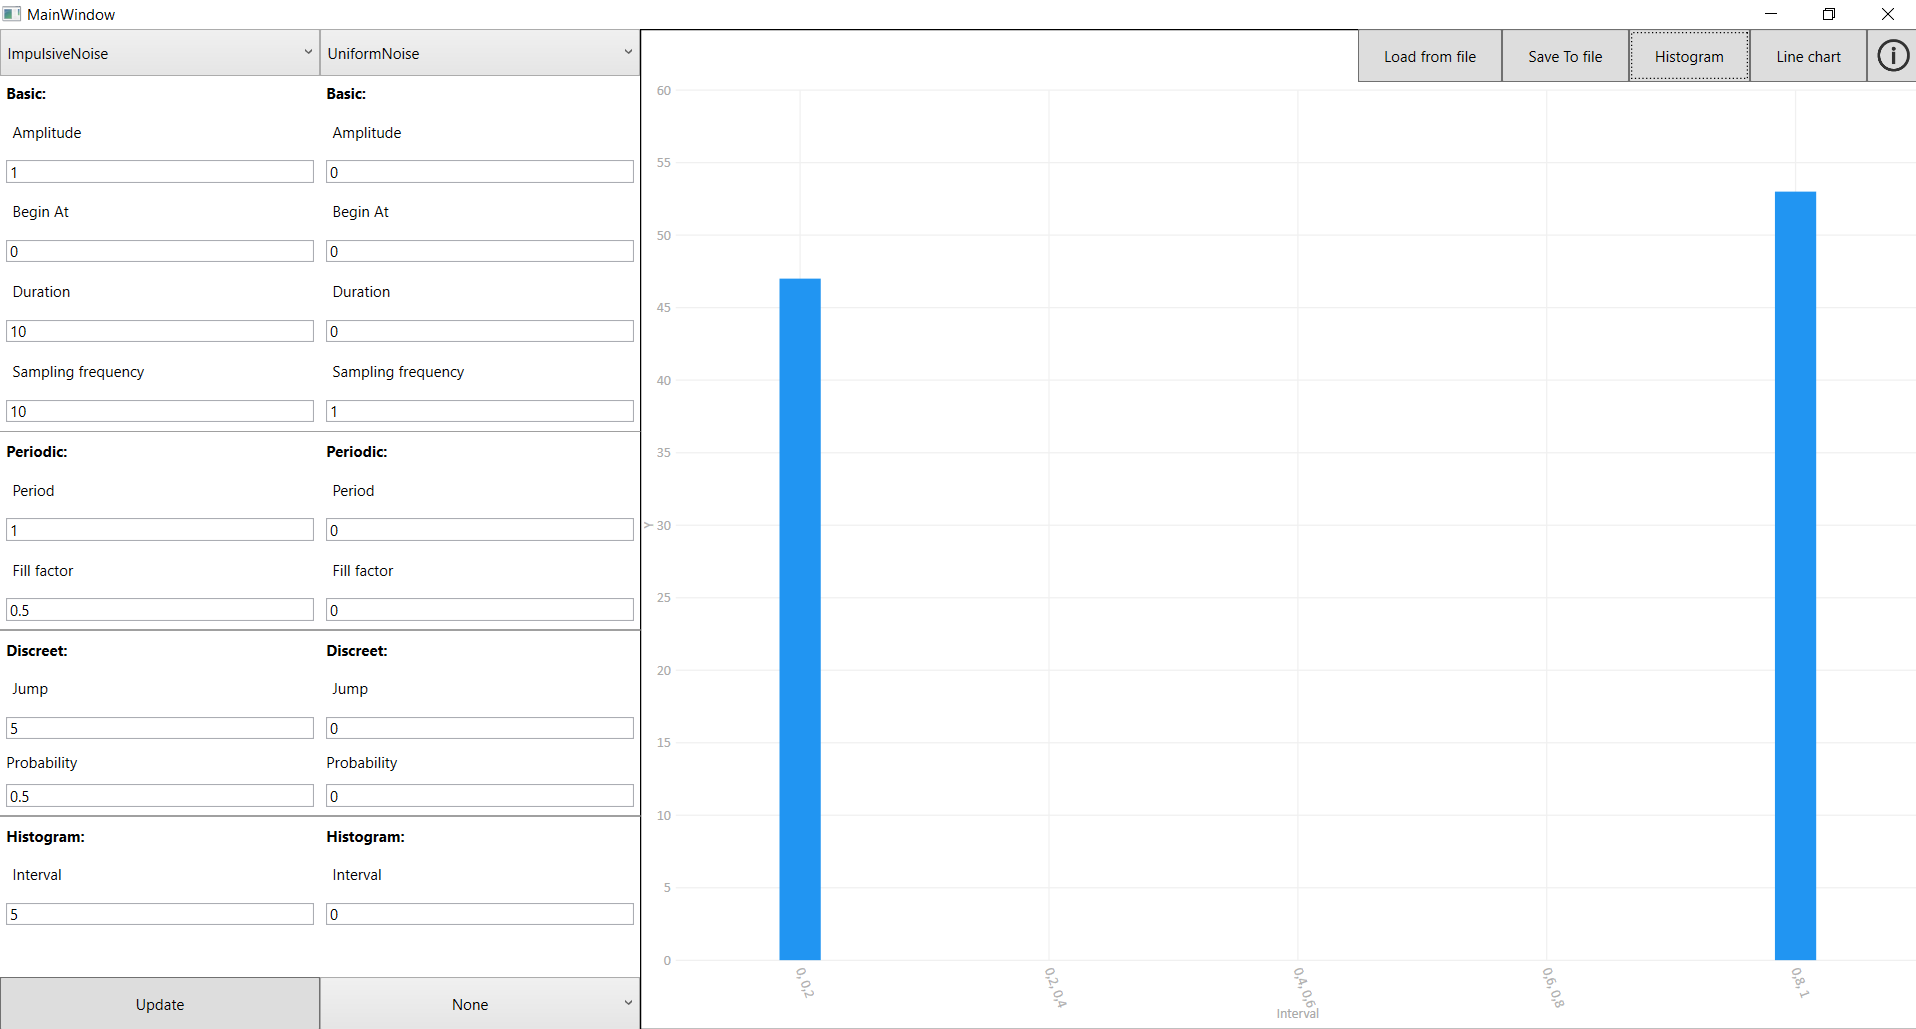
\includegraphics[width=14cm]{images/imp1hist.PNG}
 \vspace{-0.3cm}
 \caption{Histogram dla szumu impulsowego}
 \label{gui}
\end{figure}

\begin{figure}[H]
 \centering
 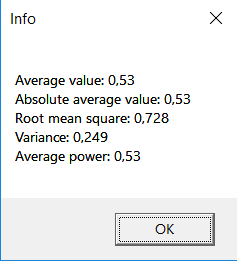
\includegraphics[width=7cm]{images/imp1info.PNG}
 \vspace{-0.3cm}
 \caption{Wyliczone wartosci dla szumu impulsowego}
 \label{gui}
\end{figure}

%%%%%%%%%%%%%%%%%%%%%%%%%%%%%%%%%%%%%%%%%%%%%%%%%%%%%%%%%%%%%%%%%%%%%%%%%%%%%%%%%%%%%%%%%%%%%%%%%%%%%%%%%%%%%%%%%
% PODROZDZIAŁ PT. EKSPERYMENT NR 12
%%%%%%%%%%%%%%%%%%%%%%%%%%%%%%%%%%%%%%%%%%%%%%%%%%%%%%%%%%%%%%%%%%%%%%%%%%%%%%%%%%%%%%%%%%%%%%%%%%%%%%%%%%%%%%%%%


\subsection{Eksperyment nr 12 }
\subsubsection{Suma sygnału sinusoidalnego i szumu gaussowskiego}
Celem tego eksperymentu było wygenerowanie sygnału będącego sumą sygnału sinusoidalnego i szumu gaussowskiego


\subsubsection{Rezultat}

\begin{figure}[H]
 \centering
 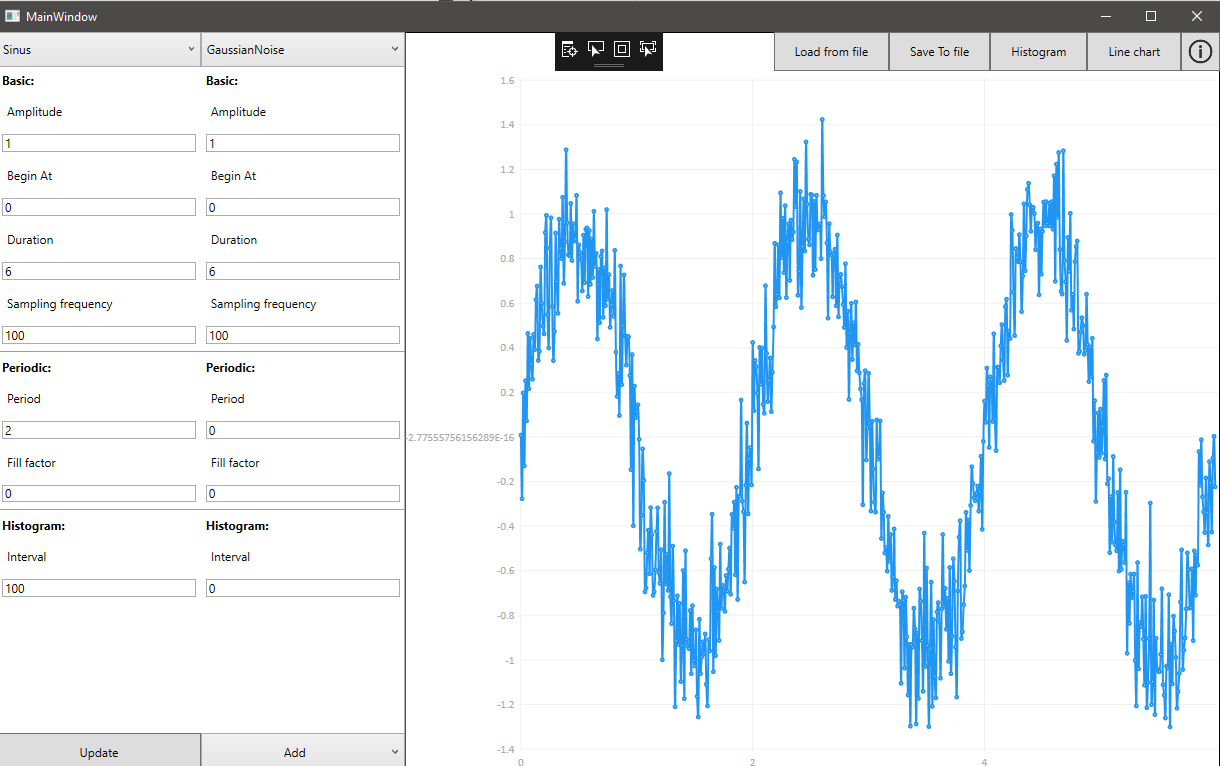
\includegraphics[width=14cm]{images/addsingauss1.PNG}
 \vspace{-0.3cm}
 \caption{Wykres sumy sygnału sinusoidalnego i szumu gaussowskiego}
 \label{gui}
\end{figure}

\begin{figure}[H]
 \centering
 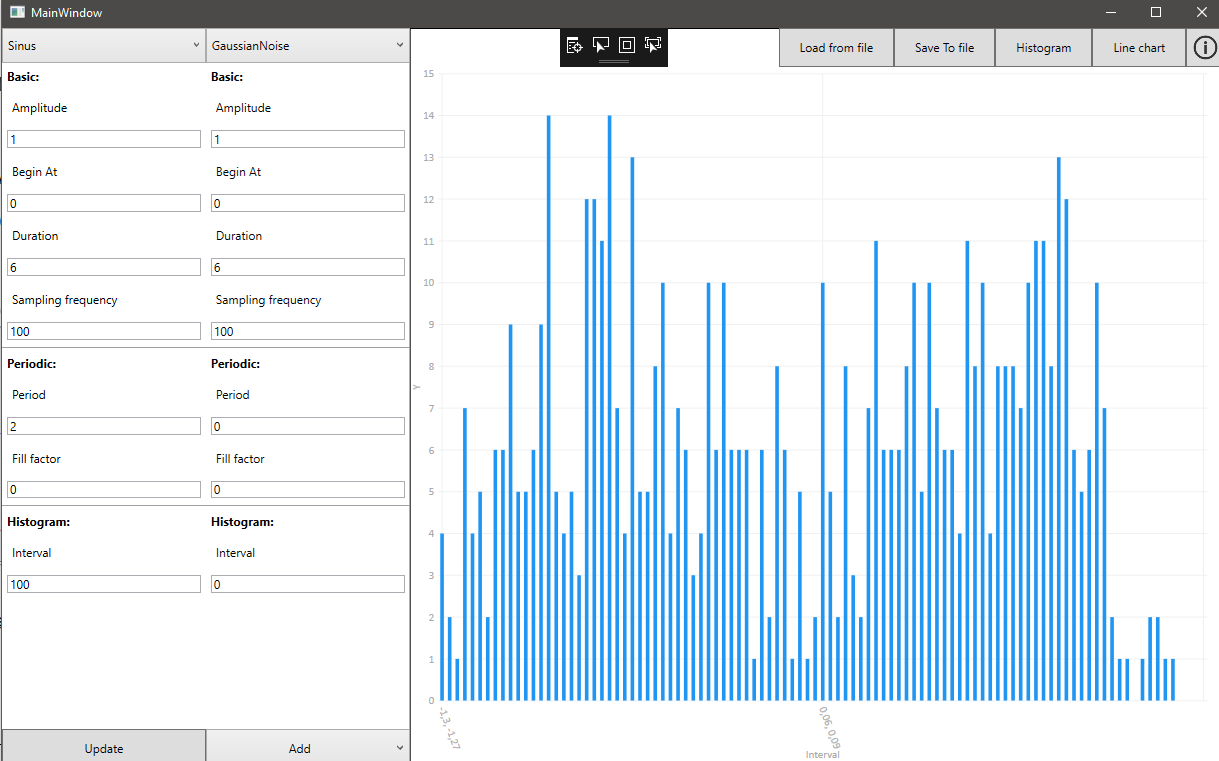
\includegraphics[width=14cm]{images/addsingauss1hist.PNG}
 \vspace{-0.3cm}
 \caption{Histogram dla  sumy sygnału sinusoidalnego i szumu gaussowskiegoo}
 \label{gui}
\end{figure}

\begin{figure}[H]
 \centering
 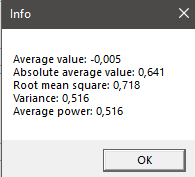
\includegraphics[width=7cm]{images/addsingauss1info.PNG}
 \vspace{-0.3cm}
 \caption{Wyliczone wartosci dla  sumy sygnału sinusoidalnego i szumu gaussowskiego}
 \label{gui}
\end{figure}

%%%%%%%%%%%%%%%%%%%%%%%%%%%%%%%%%%%%%%%%%%%%%%%%%%%%%%%%%%%%%%%%%%%%%%%%%%%%%%%%%%%%%%%%%%%%%%%%%%%%%%%%%%%%%%%%%
% PODROZDZIAŁ PT. EKSPERYMENT NR 13
%%%%%%%%%%%%%%%%%%%%%%%%%%%%%%%%%%%%%%%%%%%%%%%%%%%%%%%%%%%%%%%%%%%%%%%%%%%%%%%%%%%%%%%%%%%%%%%%%%%%%%%%%%%%%%%%%


\subsection{Eksperyment nr 13 }
\subsubsection{Iloczyn sygnału sinusoidalnego wyprostowanego dwupołówkowo i sygnału 
kątnego}
Celem tego eksperymentu było wygenerowanie sygnału będącego iloczynem sygnału sinusoidalnego wyprostowanego dwupołówkowo i sygnału trójkątnego.


\subsubsection{Rezultat}

\begin{figure}[H]
 \centering
 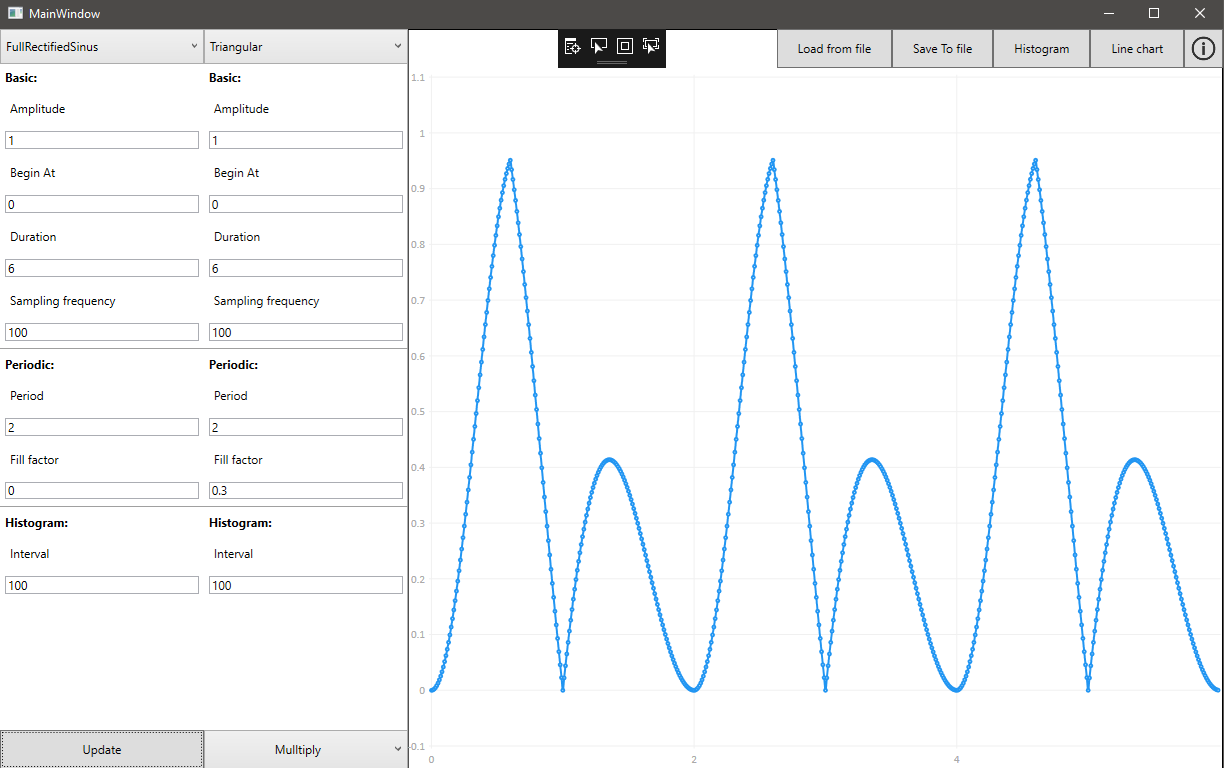
\includegraphics[width=14cm]{images/mulfulltrian1.PNG}
 \vspace{-0.3cm}
 \caption{Wykres  iloczynu sygnału sinusoidalnego wyprostowanego dwupołówkowo i sygnału trójkątnego}
 \label{gui}
\end{figure}

\begin{figure}[H]
 \centering
 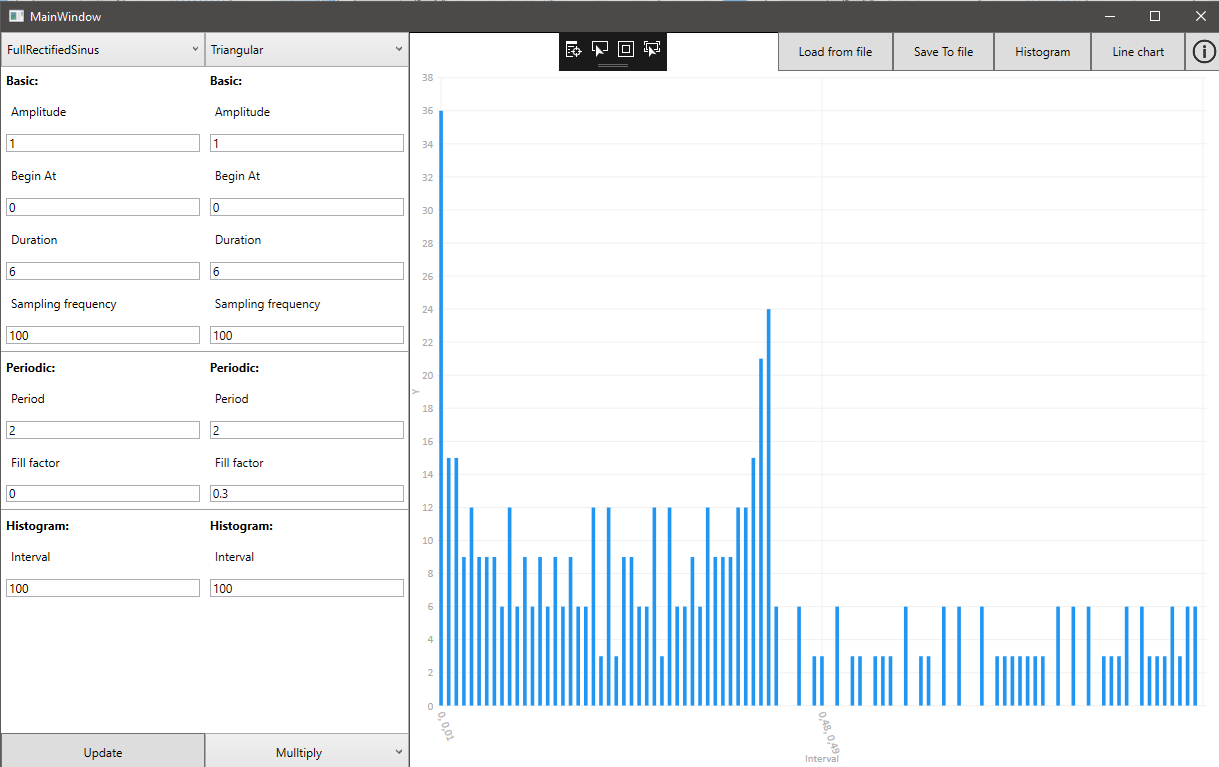
\includegraphics[width=14cm]{images/mulfulltrian1hist.PNG}
 \vspace{-0.3cm}
 \caption{Histogram dla iloczynu sygnału sinusoidalnego wyprostowanego dwupołówkowo i sygnału trójkątnego}
 \label{gui}
\end{figure}

\begin{figure}[H]
 \centering
 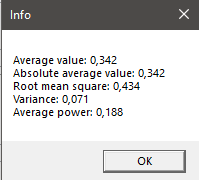
\includegraphics[width=7cm]{images/mulfulltrian1info.PNG}
 \vspace{-0.3cm}
 \caption{Wyliczone wartosci dla iloczynu sygnału sinusoidalnego wyprostowanego dwupołówkowo i sygnału trójkątnego}
 \label{gui}
\end{figure}



\newpage

\section{Wnioski}

Aplikacja została napisania zgodnie z instrukcją zadania \cite{zad}. Aplikacja pozwala na rozszerzanie jej o kolejne funkcjonalnosci na potrzeby kolejnych zadań. 




%%%%%%%%%%%%%%%%%%%%%%%%%%%%%%%%%%%%%%%%%%%%%%%%%%%%%%%%%%%%%%%%%%%%%%%%%%%%%%%%%%%%%%%%%%%%%%%%%%%%%%%%%%%%%%%%%
% BIBLIOGRAFIA
%%%%%%%%%%%%%%%%%%%%%%%%%%%%%%%%%%%%%%%%%%%%%%%%%%%%%%%%%%%%%%%%%%%%%%%%%%%%%%%%%%%%%%%%%%%%%%%%%%%%%%%%%%%%%%%%%

\begin{thebibliography}{99}
\bibitem{pa} H.~Partl:
\emph{German \TeX},
TUGboat Vol.~9,, No.~1 ('88)
\bibitem{lv} Biblioteka LiveCharts. https://lvcharts.net
\bibitem{wpf} Windows Presentation Foundation. https://docs.microsoft.com/plpl/dotnet/framework/wpf/getting-started/walkthrough-my-frst-wpfdesktop-application
\bibitem{zad} Tresć zadania https://ftims.edu.p.lodz.pl/file.php/154/zadanie1\_20101011.pdf
\end{thebibliography}

\end{document}
